\chapter{Đánh giá các thông số hiệu năng của mô hình nhận diện}
Mô hình được huấn luyện trong ba ngày với $12000$ iteration. Trong quá trình huấn luyện, việc tính toán các thông số hiệu năng của mô hình được thực hiện với mỗi $1000$ iteration trên tập dữ liệu validation. 
Nhắc lại về cách tính các thông số hiệu năng:
\begin{itemize}
	\item Precision là thông số thể hiện độ chính xác của các dự đoán. $True Positive$ (viết tắt: TP) là những bounding box được dán nhãn đúng và thực sự đúng. $False Positive$ (viết tắt: FP) là những bounding box được dán nhãn đúng và không thực sự đúng. Precision được tính bằng công thức
	\begin{equation}
		precision = \frac{TP}{TP+FP}
	\end{equation}
	\item Recall là thông số thể hiện độ nhạy của mô hình với các đối tượng cần nhận dạng. $True Positive$ (viết tắt: TP) là những bounding box được dán nhãn đúng và thực sự đúng. $False Negative$ (viết tắt: FN) là những bounding box được dán nhãn không đúng hoặc không được dán nhãn và thực sự đúng. Recall được tính bằng công thức
	\begin{equation}
		precision = \frac{TP}{TP+FN}
	\end{equation}
	\item Average precision là thông số được tính cho một class. Với mỗi class, trong quá trình đánh giá trên tập dữ liệu validation, các giá trị precision và recall sẽ được lưu lại. Sau đó ta sẽ vẽ đồ thị của precision theo recall, average precision của một class sẽ là phần diện tích dưới đồ thị này. Gọi $p(r):[0,1]\rightarrow[0,1]$ là hàm số biểu diễn quan hệ của precision và recall. Average precision của một class sẽ được tính theo công thức
	\begin{equation}
		\text{average precision} = \int_{0}^{1} p(r) dr
	\end{equation}
	\item Mean average precision là trung bình của các average precision của các class
	\begin{equation}
		\text{mean average precision} = \frac{\sum_{i=0}^{N} ap_i}{N}
	\end{equation}
	Với $N \in \mathbb{N}^*$ là số class của mô hình.
\end{itemize}

Tập dữ liệu validation gồm $900$ hình được chia một cách ngẫu nhiên từ tập dữ liệu gốc và không được dùng để huấn luyện, số lượng các object trong tập dữ liệu này được thể hiện trong hình \ref{fig:validation_set}
\begin{figure}[ht!]
	\centerline{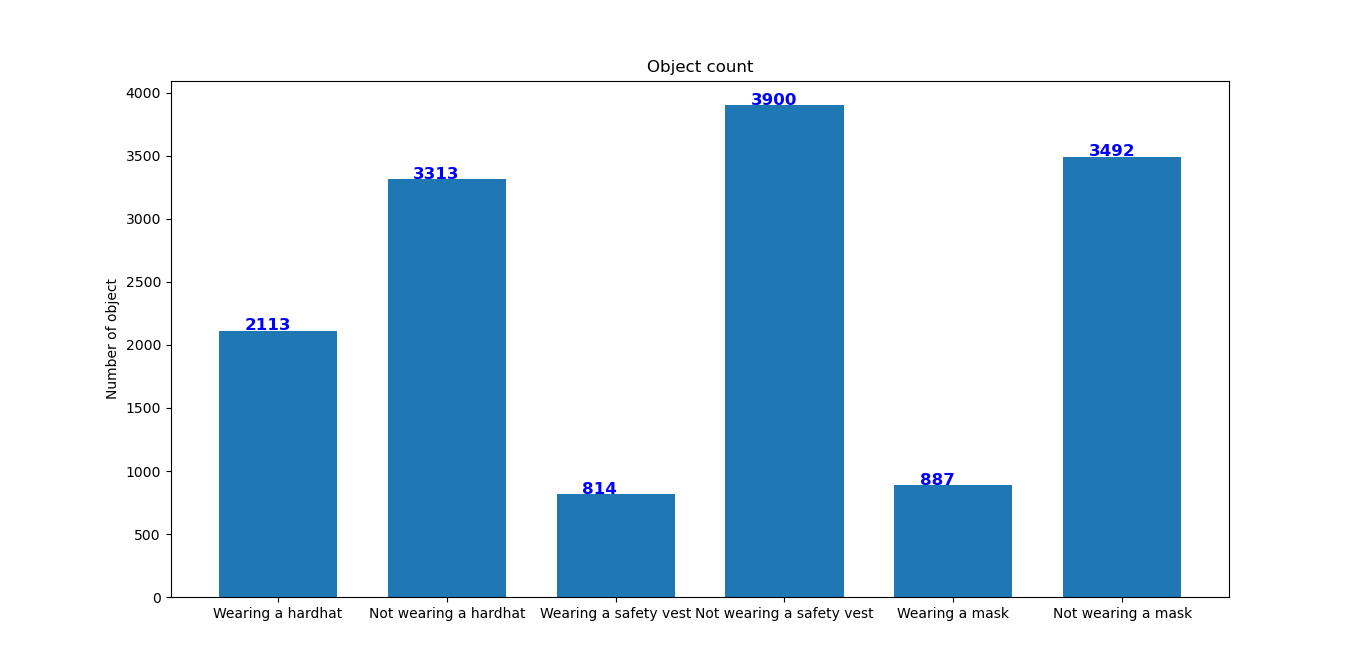
\includegraphics[scale=0.5]{images/validation_set.png}}
  	\caption{Số lượng các object trong tập dữ liệu validation. Wearing a hardhat - $2113$, Not wearing a hardhat - $3313$, Wearing a safety vest - $814$, Not wearing a safety vest - $3900$, Wearing a mask - $887$, Not wearing a mask - $3492$.}
  	\label{fig:validation_set}
\end{figure}

Các thông số được tính toán gồm: precision, recall và mean average precision \ref{fig:precision_recall_map}.
\begin{figure}[ht!]
	\centerline{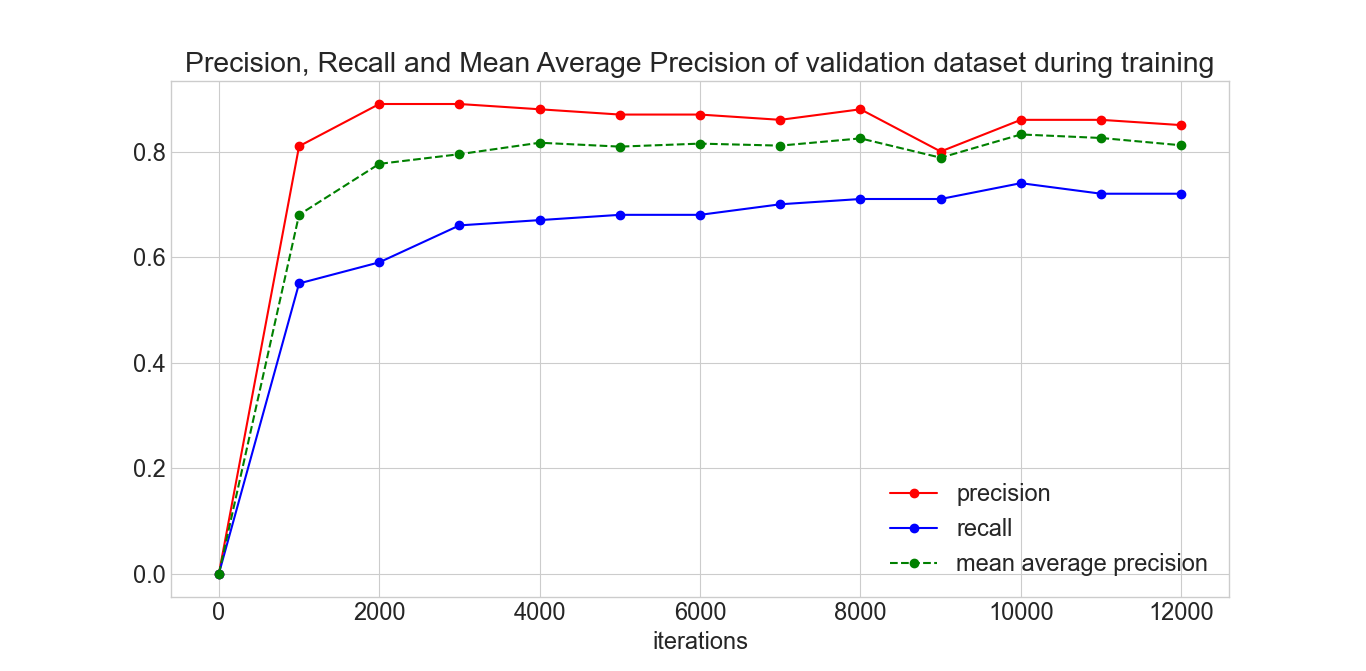
\includegraphics[scale=0.5]{images/precision_recall_map.png}}
  	\caption{Precision - màu đỏ, Recall - màu xanh dương, Mean Average Precision - màu xanh lá. Các thông số được tính toán mỗi 1000 iteration trên tập dữ liệu validation.}
  	\label{fig:precision_recall_map}
\end{figure}

\subsection{Thử nghiệm mô hình trong các trường hợp thực tế}
Việc đánh giá mô hình trên tập dữ liệu validation cũng phần nào phản ánh được các thông số hiệu năng của mô hình, tuy nhiên để có thể có những đánh giá trực quan hơn, cần thiết phải có những kiểm nghiệm thực tế. Các bài kiểm tra sau được thực hiện trong các điều kiện và hoàn cảnh khác nhau nhằm khảo sát khả năng dự đoán của mô hình trong các trường hợp có thể xảy ra. Mỗi trường hợp sẽ được chụp một số hình ảnh nhất đình, sau đó sẽ tiến hành dùng mô hình để dự đoán trên các hình ảnh này, sau cùng là đánh giá các thông số hiệu năng của mô hình trong các trường hợp. Các hình ảnh được chụp từ camera có khẩu độ f 4.0, tiêu cự 14 mm.
\subsubsection{Khảo sát về precission và recall của mô hình khi khoảng cách từ camera đến các chủ thể thay đổi}
Trong thử nghiệm này các chủ thể sẽ đứng lần lượt ở các khoảng cách $3$m - hình \ref{fig:3m}, $6$m - hình \ref{fig:6m} và $9$m - hình \ref{fig:9m} so với camera. 
\begin{figure}[ht!]% [H] is so declass\'e!
\centering
\begin{minipage}{0.45\textwidth}
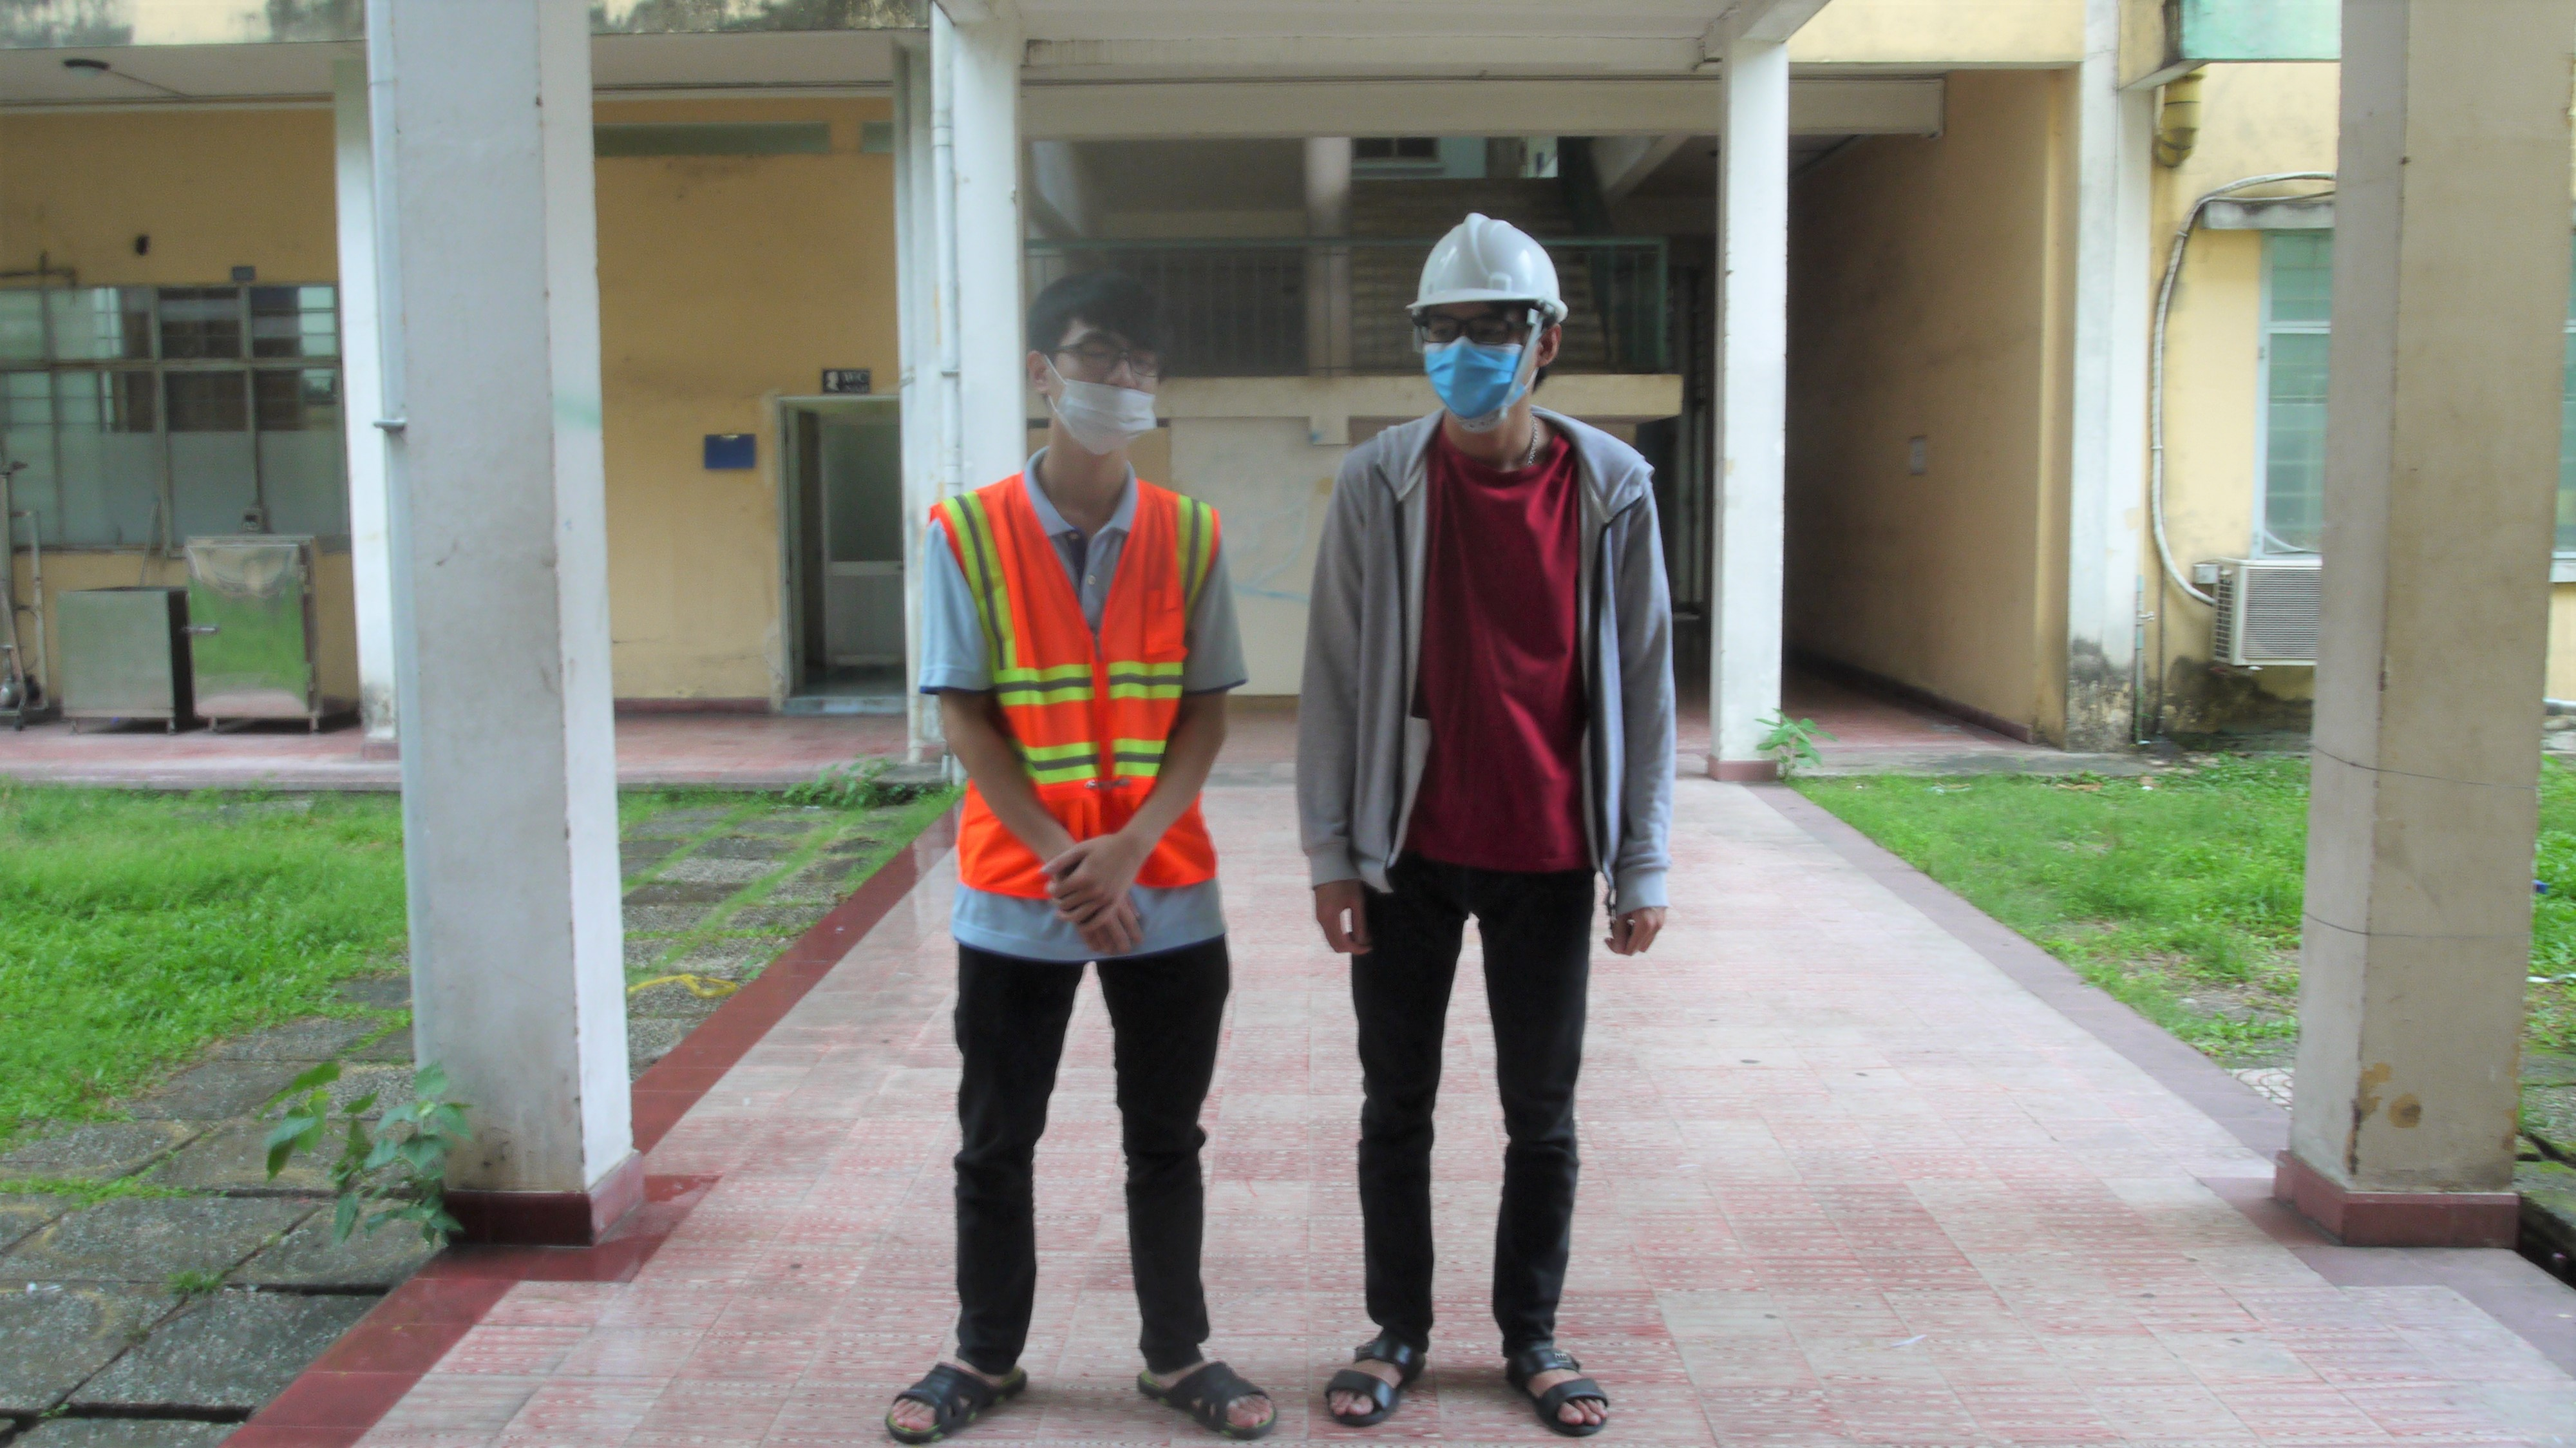
\includegraphics[width=\textwidth]{images/3m1.JPG}
\caption{Các chủ thể đứng cách camera ở khoảng cách 3m.}
\label{fig:3m}
\end{minipage}\hfill
\begin{minipage}{0.45\textwidth}
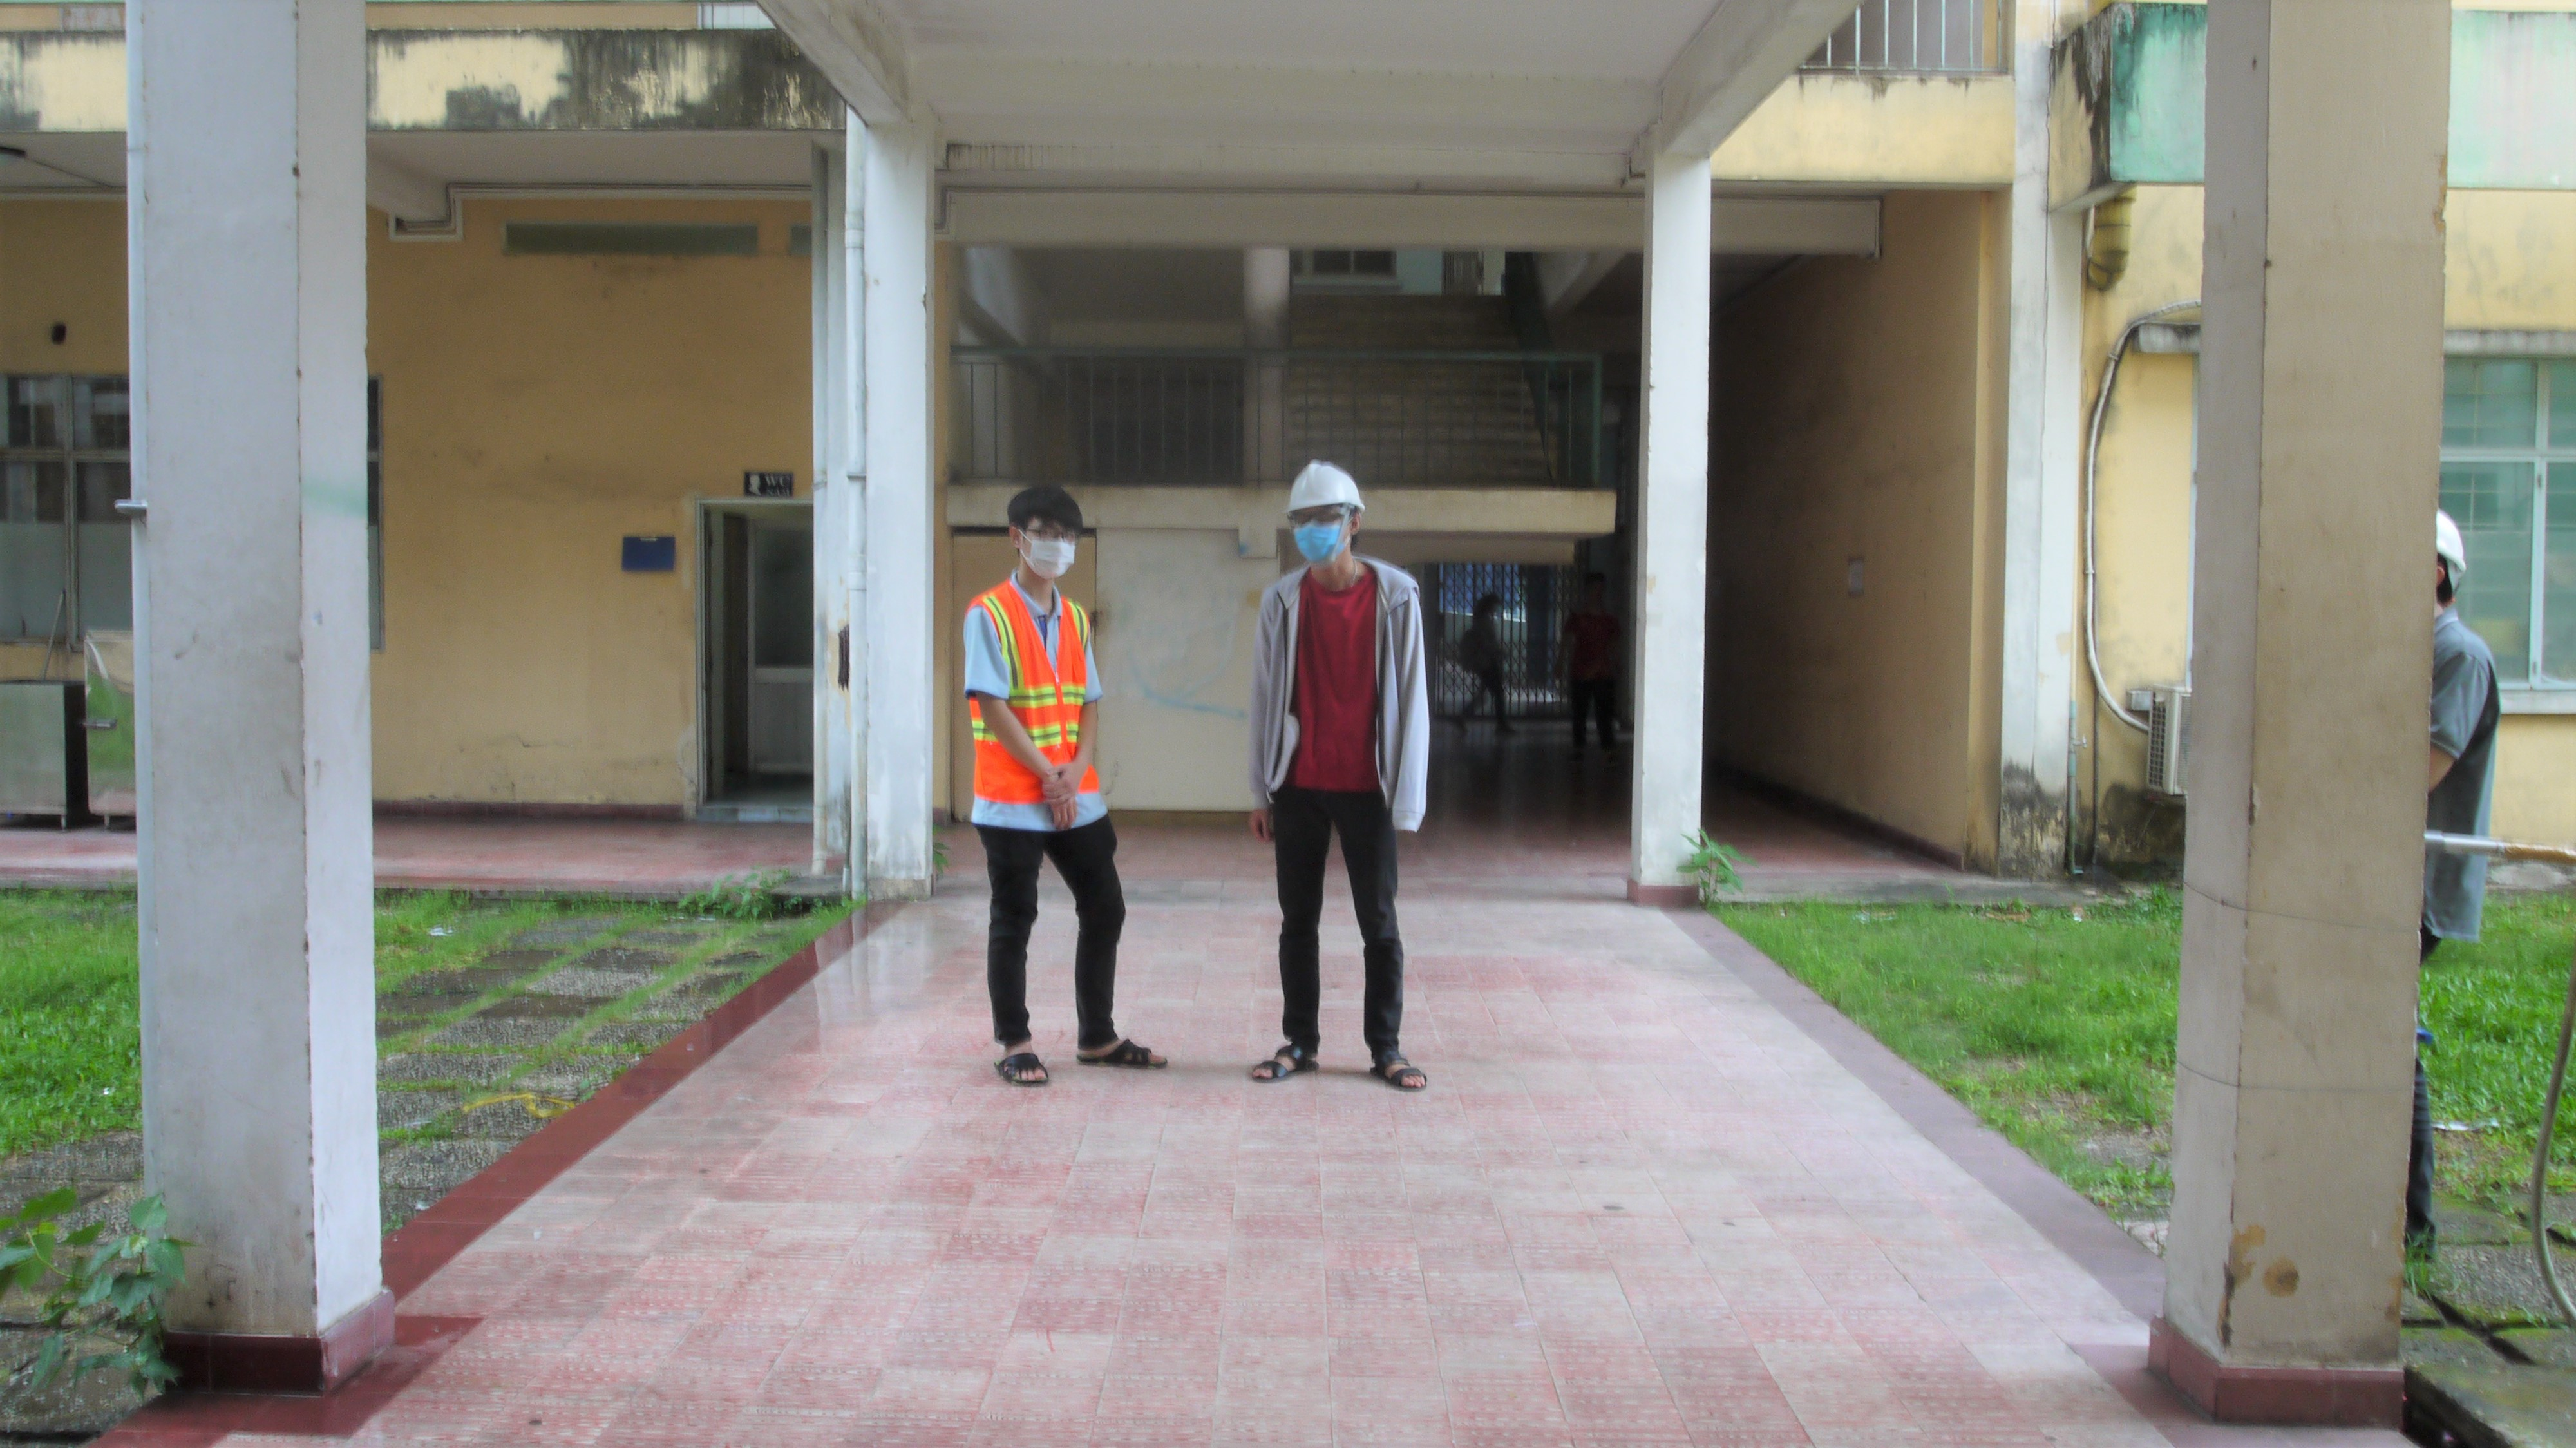
\includegraphics[width=\textwidth]{images/6m1.JPG}
\caption{Các chủ thể đứng cách camera ở khoảng cách 6m.}
\label{fig:6m}
\end{minipage}\par
\vskip\floatsep% normal separation between figures
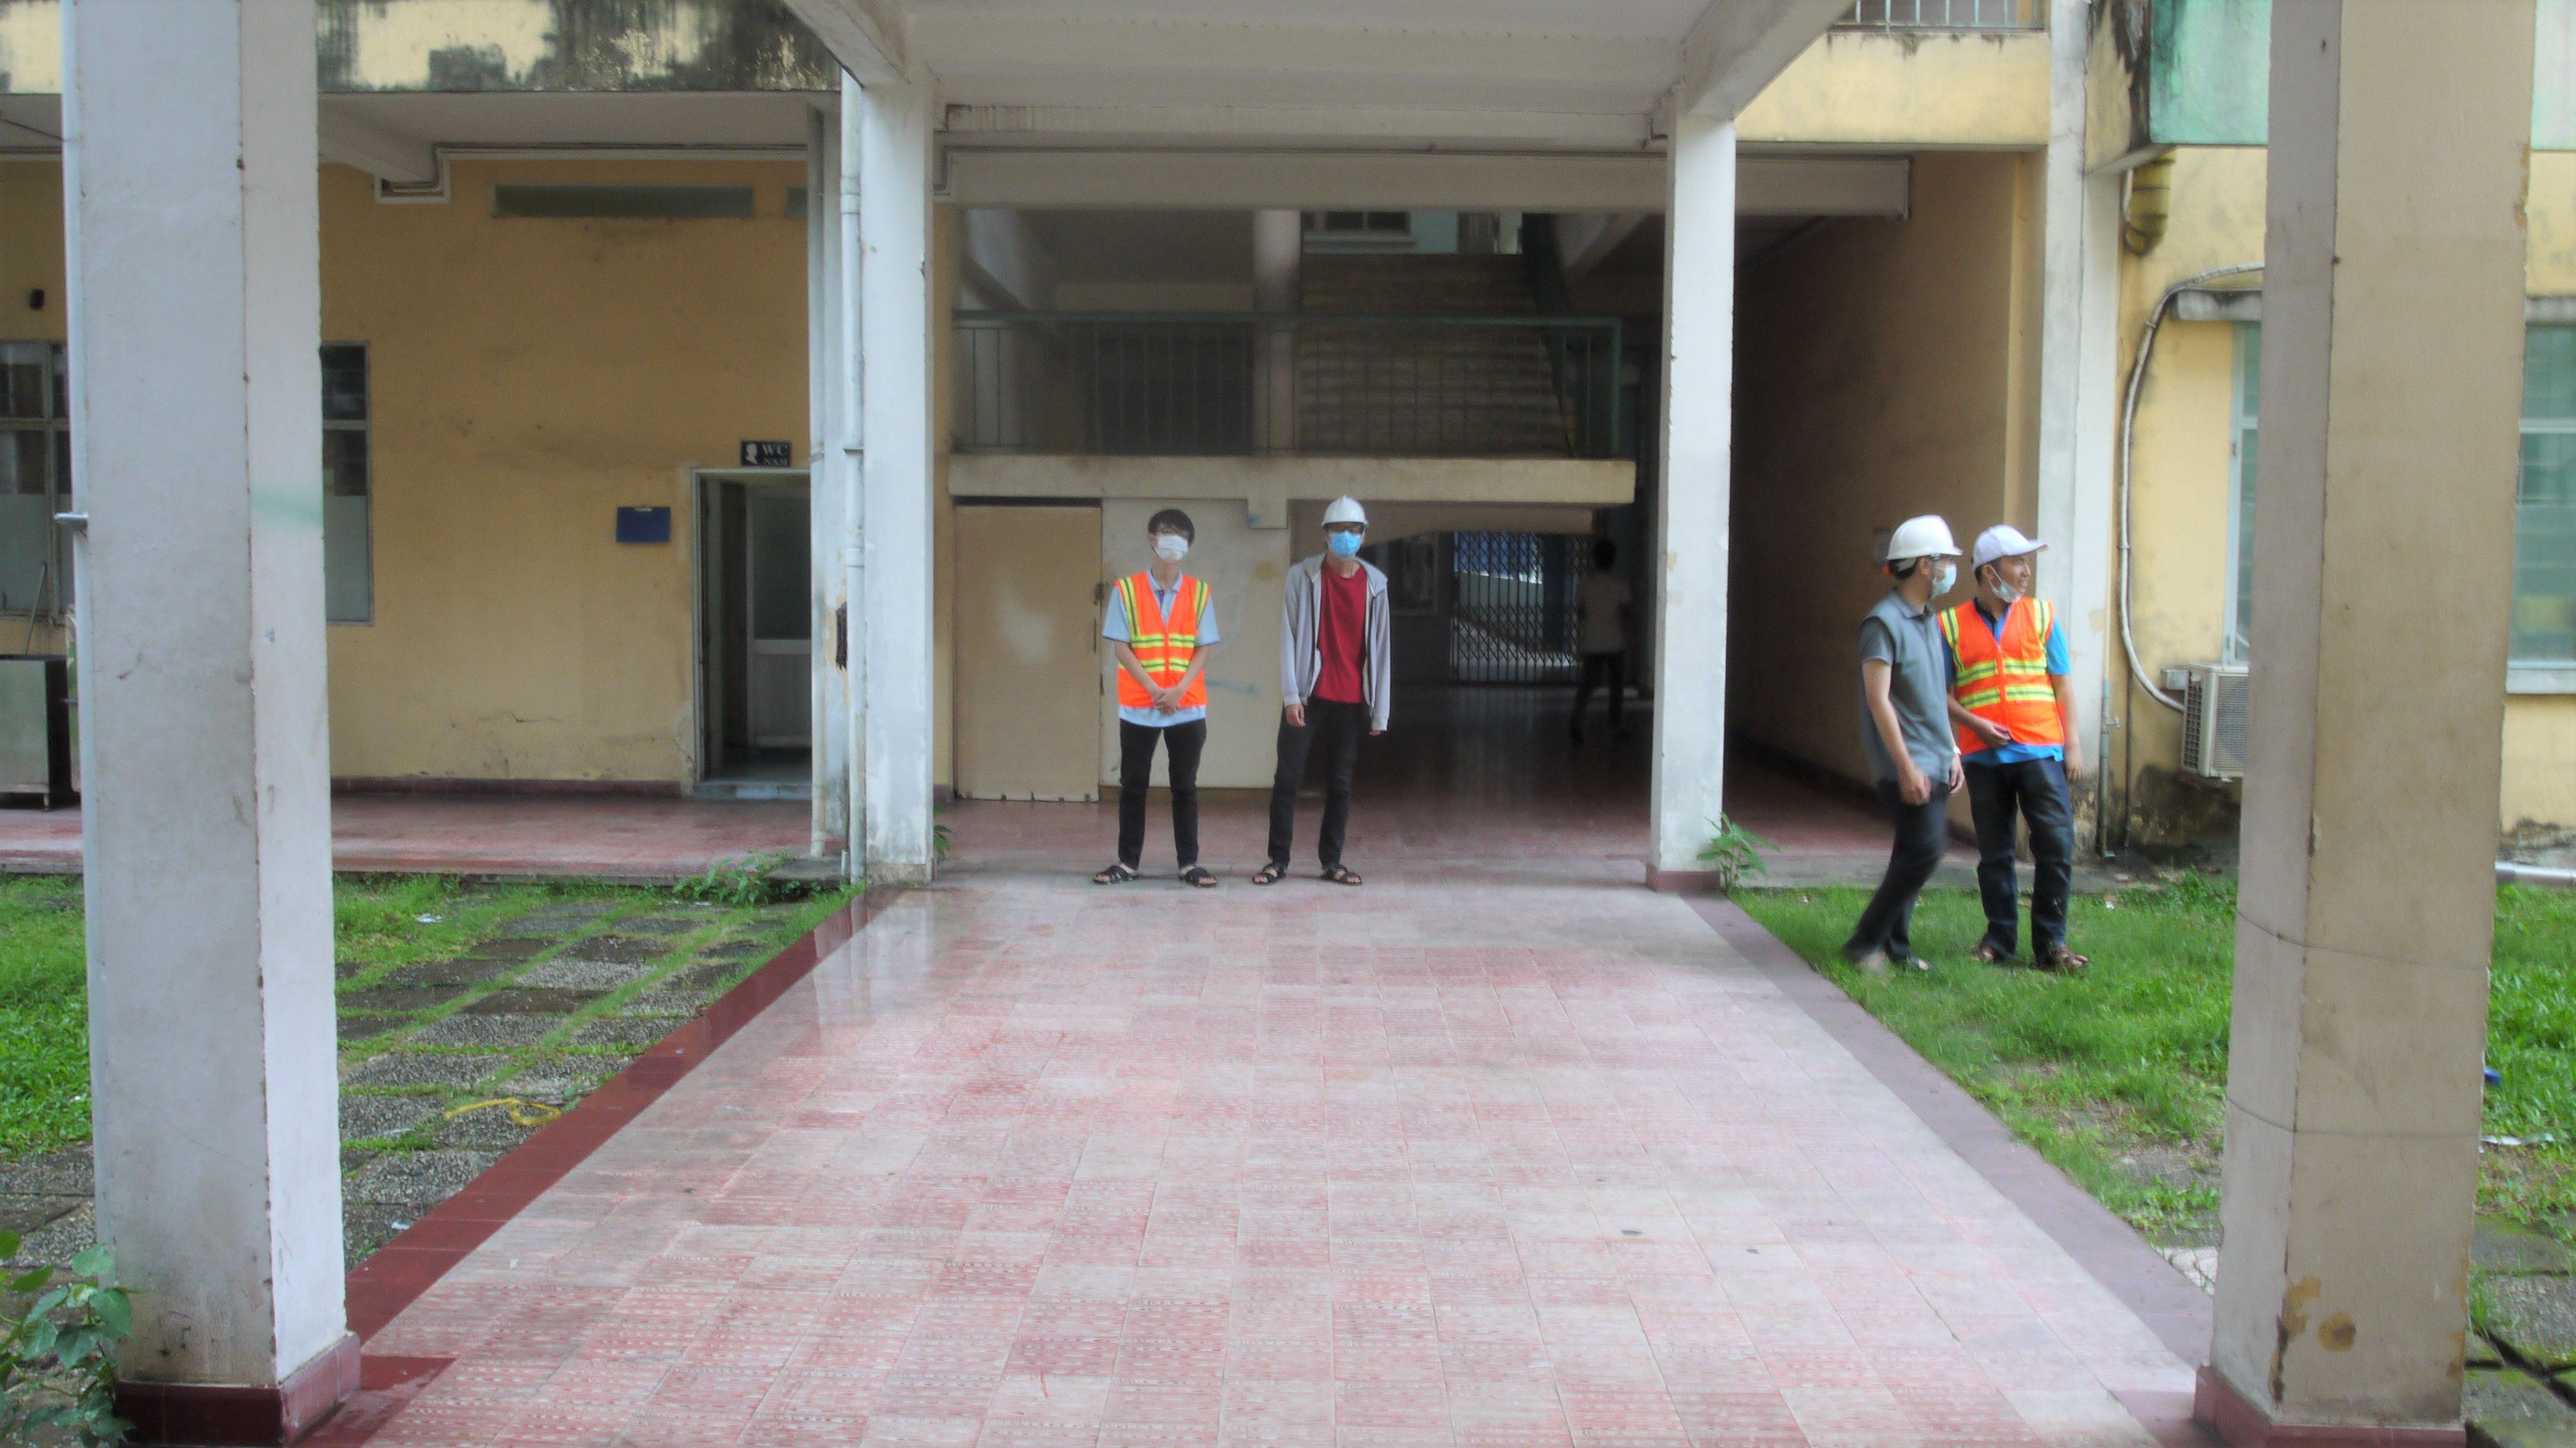
\includegraphics[width=0.45\textwidth]{images/9m1.JPG}
\caption{Các chủ thể đứng cách camera ở khoảng cách 9m.}
\label{fig:9m}
\end{figure}
Ngoài ra sẽ có một chủ thể sử dụng nón vải màu trắng, gần giống với nón bảo hiểm màu trắng - hình \ref{fig:similar_white_hat_1} và hình \ref{fig:similar_white_hat_2} để kiểm nghiệm khả năng phân biệt các vật thể gần giống nhau của mô hình.
\begin{figure}[ht!]% [H] is so declass\'e!
\centering
\begin{minipage}{0.45\textwidth}
\includegraphics[width=\textwidth]{images/close1.JPG}
\caption{Một chủ thể đội nón vải trắng - bên trái và một chủ thể đội nón bảo hiểm trắng - bên phải. Góc chụp trực diện}
\label{fig:similar_white_hat_1}
\end{minipage}\hfill
\begin{minipage}{0.45\textwidth}
\includegraphics[width=\textwidth]{images/close2.JPG}
\caption{Một chủ thể đội nón vải trắng - bên trái và một chủ thể đội nón bảo hiểm trắng - bên phải. Góc chụp từ trái qua}
\label{fig:similar_white_hat_2}
\end{minipage}
\end{figure}

\emph{Kết quả}: Đồ thị precision ở hình \ref{fig:3_6_9_precision} và recall ở hình \ref{fig:3_6_9_recall} cho thấy mô hình hoạt động tốt nhất ở khoảng cách $6$m. Các thông số precision và recall của hầu hết các class ở $6$m đều trội hơn so với ở $3$m và $9$m. Việc precision cao sẽ giúp các dự đoán của mô hình tại $6$m chính xác hơn so với tại $3$m và $9$m. Recall cao nói lên rằng mô hình sẽ nhạy hơn và có thể phát hiện được nhiều vật thể hơn trong một khung hình tại khoảng cách $6$m. Tại class \emph{Not wearing a hardhat} có sự dao động về thông số hiệu năng và kết quả dự đoán ở khoảng cách $6$m vẫn chưa là tốt nhất điều này có thể xuất phát từ việc các bounding box của class \emph{Not wearing a hardhat} trong tập dữ liệu huấn luyện có kích thước gần tương đồng với các bounding box của vật thể cùng class ở khoảng cách $9$m.
\begin{figure}[ht!]
	\centerline{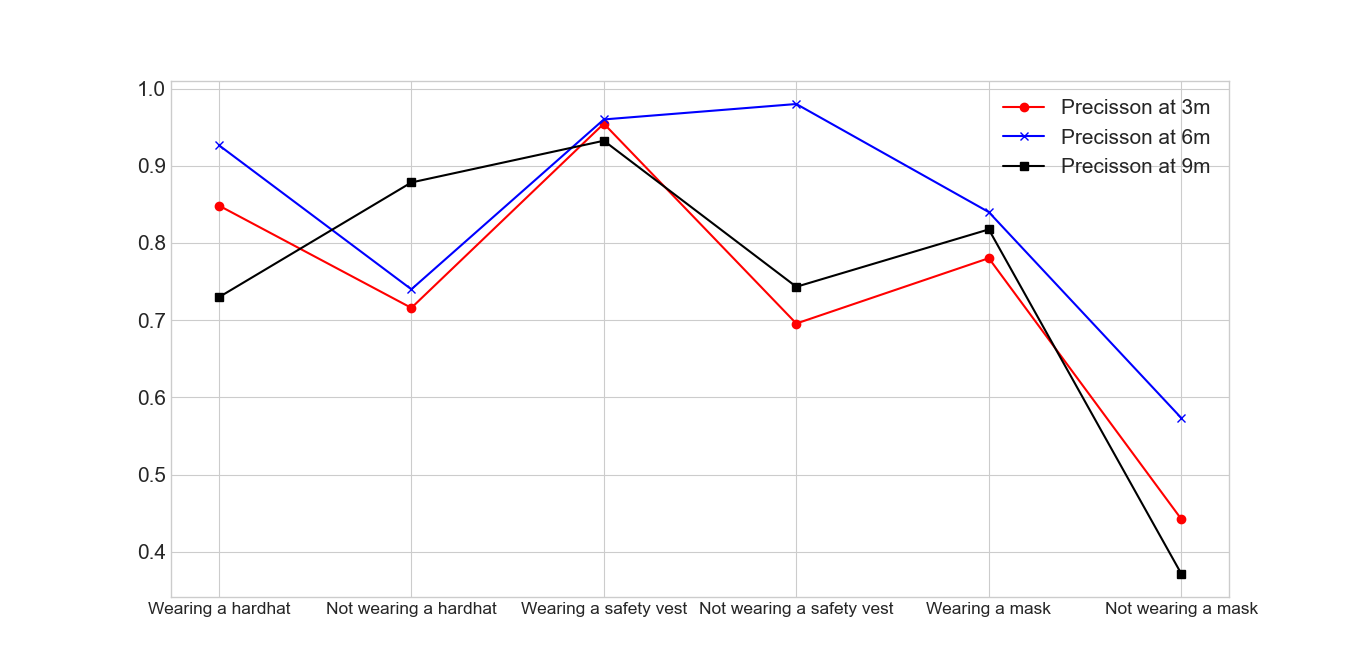
\includegraphics[scale=0.5]{images/3_6_9_precision.png}}
  	\caption{Precision của các class tại các khoảng cách {\color{red} 3m}, {\color{blue} $6$m}, {\color{black} $9$m}. Cao hơn nghĩa là tốt hơn.}
  	\label{fig:3_6_9_precision}
\end{figure}
\begin{figure}[ht!]
	\centerline{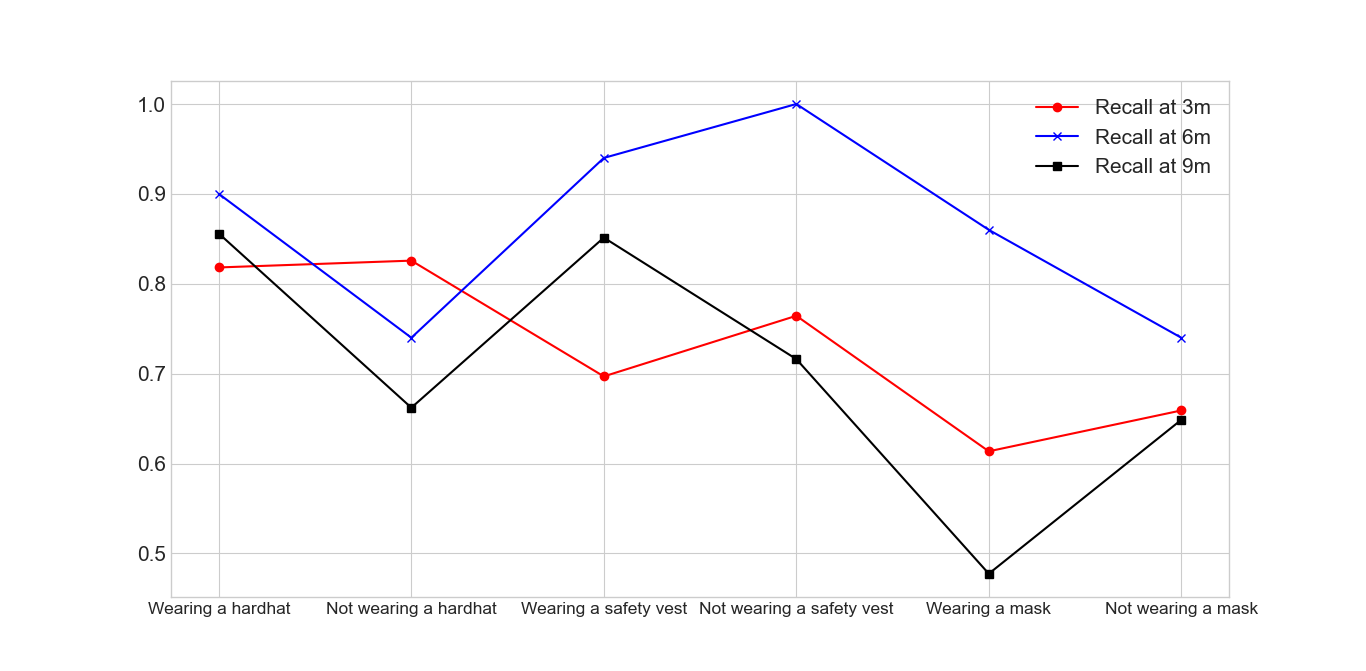
\includegraphics[scale=0.5]{images/3_6_9_recall.png}}
  	\caption{Recall của các class tại các khoảng cách {\color{red} 3m}, {\color{blue} $6$m}, {\color{black} $9$m}. Cao hơn nghĩa là tốt hơn.}
  	\label{fig:3_6_9_recall}
\end{figure}

Ngoài ra, mô hình cũng có thể phân biệt tốt giữa nón vải trắng và nón bảo hộ trắng tại khoảng cách $3$m như trên hình \ref{fig:good_hh} và \ref{fig:good_hh_zoom}. Tại $6$m mô hình vẫn tiếp tục phân biệt tốt như trên hình \ref{fig:good_hh_6m} và \ref{fig:good_hh_6m_zoom}. Độ chính xác giảm xuống khi chủ thể cách xa camera $9$m như trên hình \ref{fig:good_hh_9m} và \ref{fig:good_hh_9m_zoom}.
\begin{figure}[ht!]
	\centerline{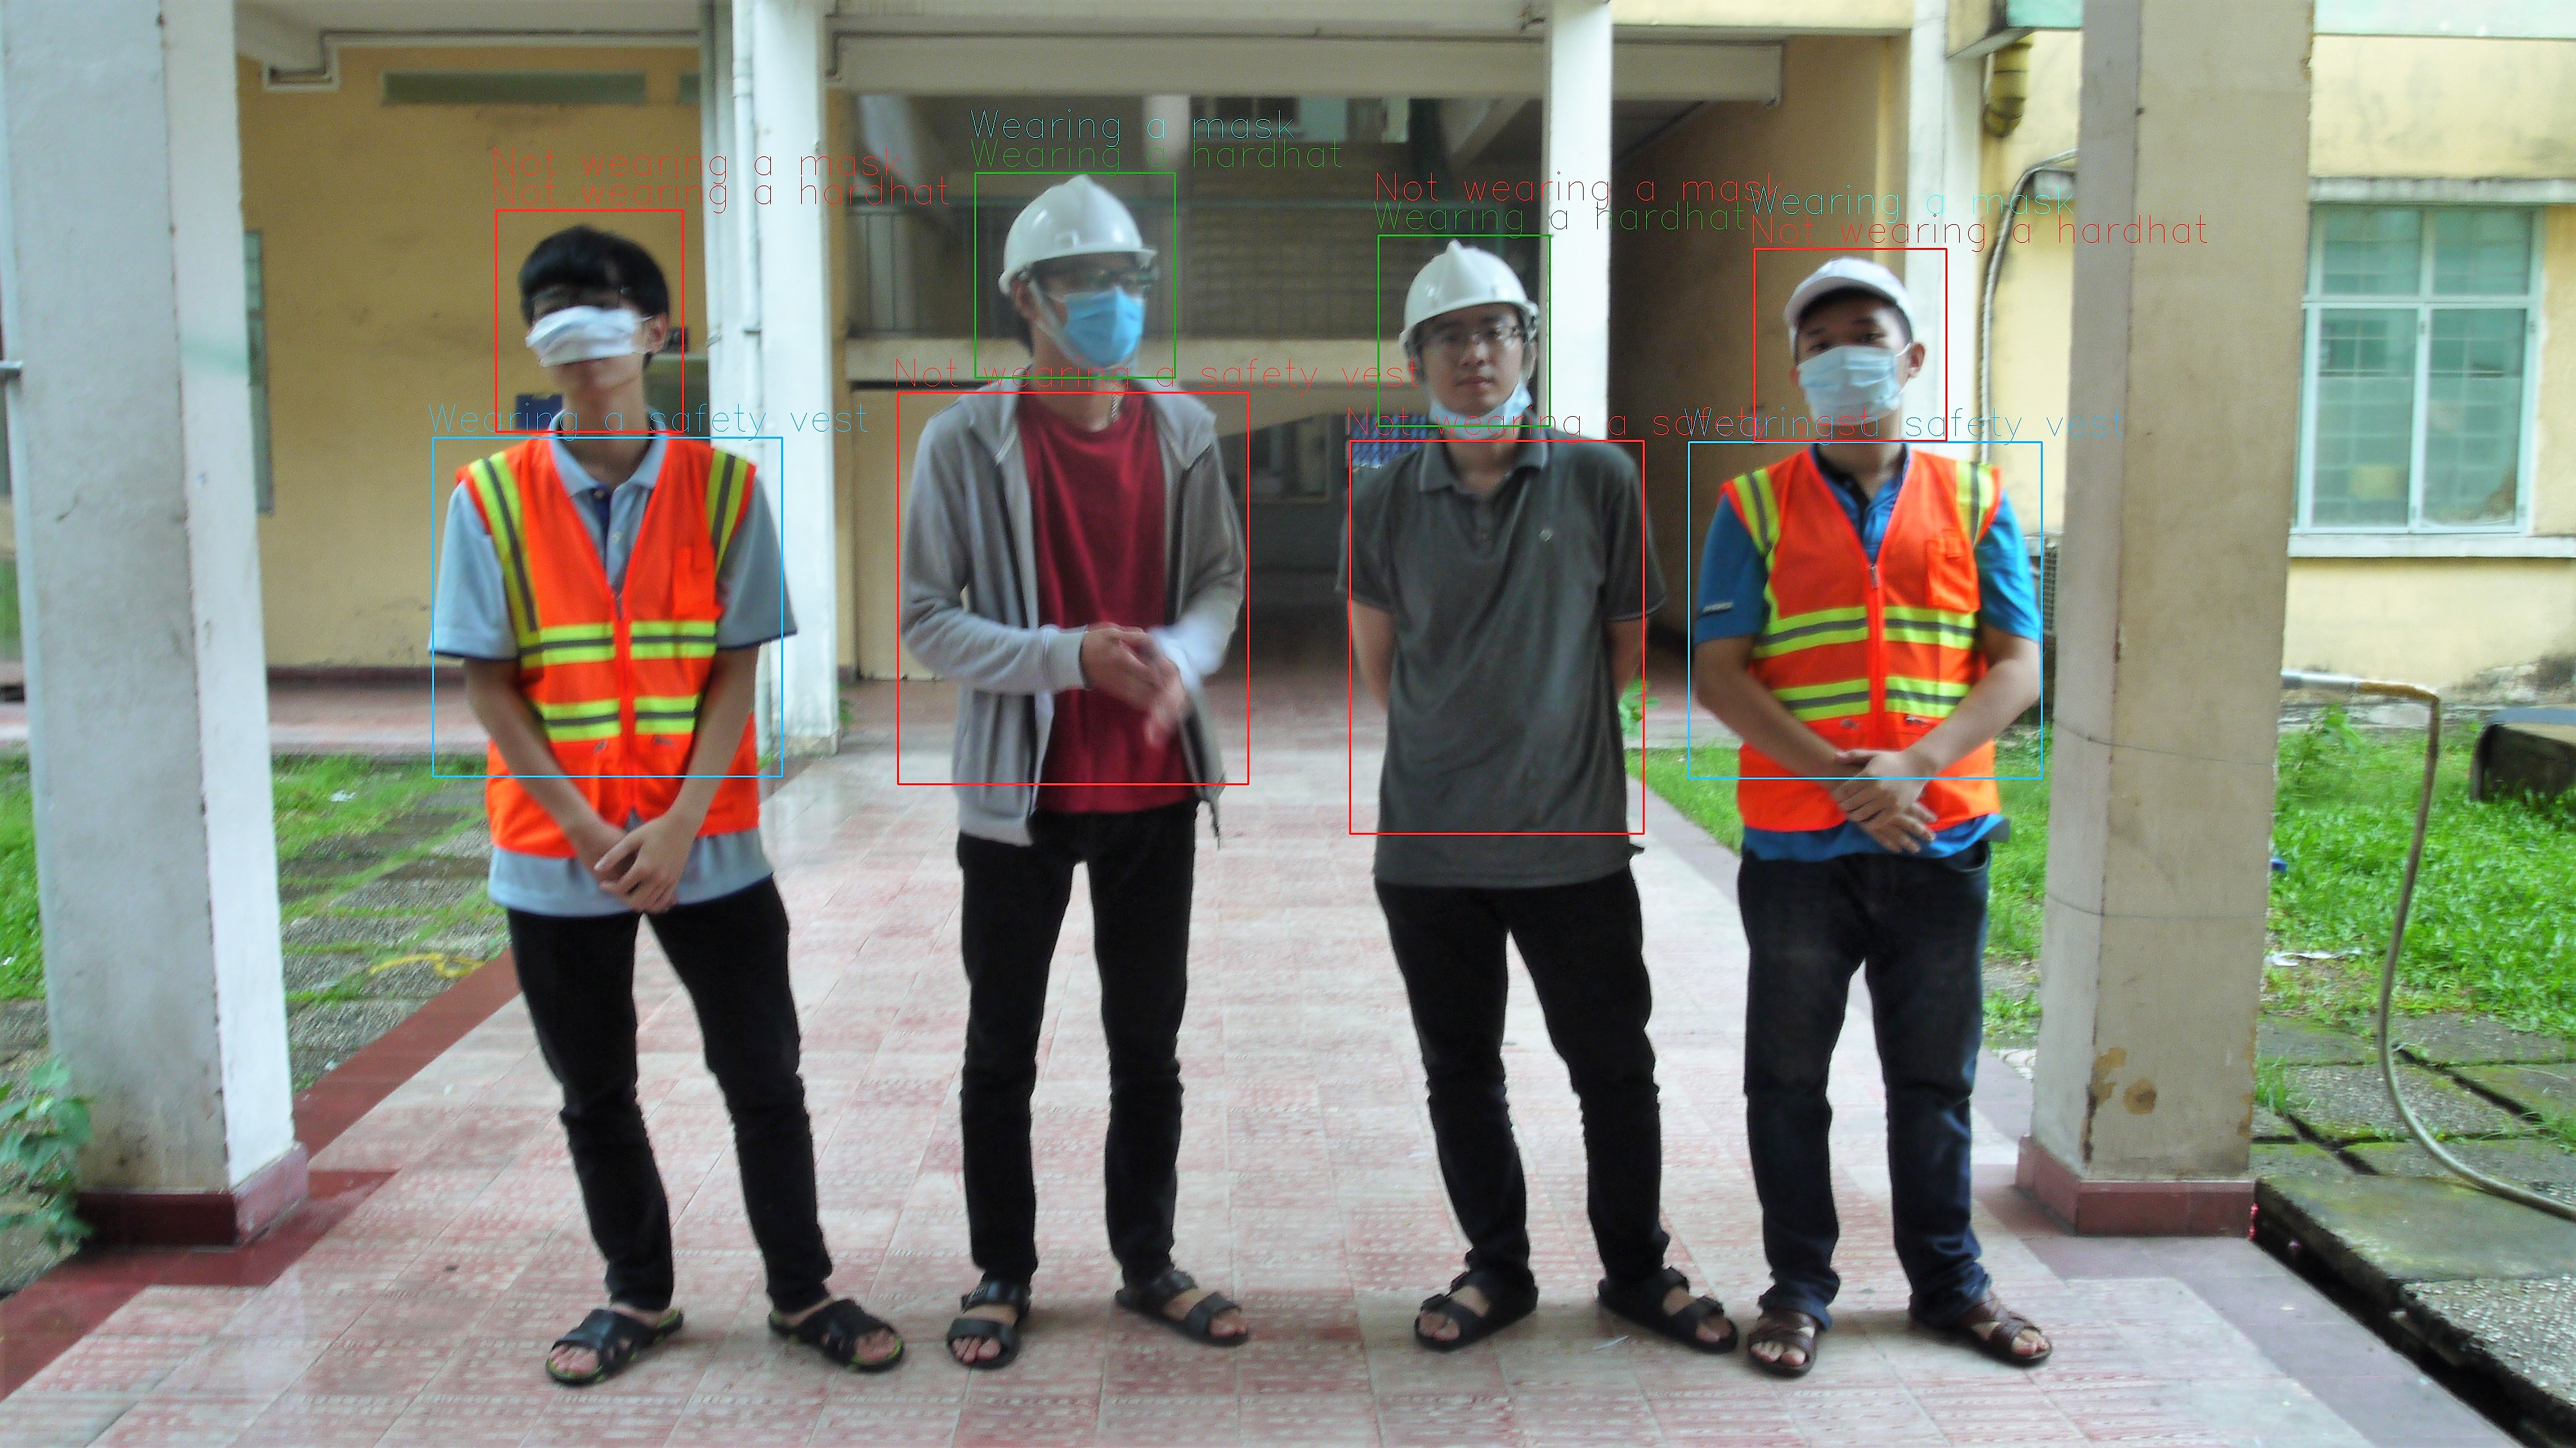
\includegraphics[scale=0.1]{images/good_hh.jpg}}
  	\caption{Dự đoán của mô hình ở khoảng cách 3m.}
  	\label{fig:good_hh}
\end{figure}
\begin{figure}[ht!]
	\centerline{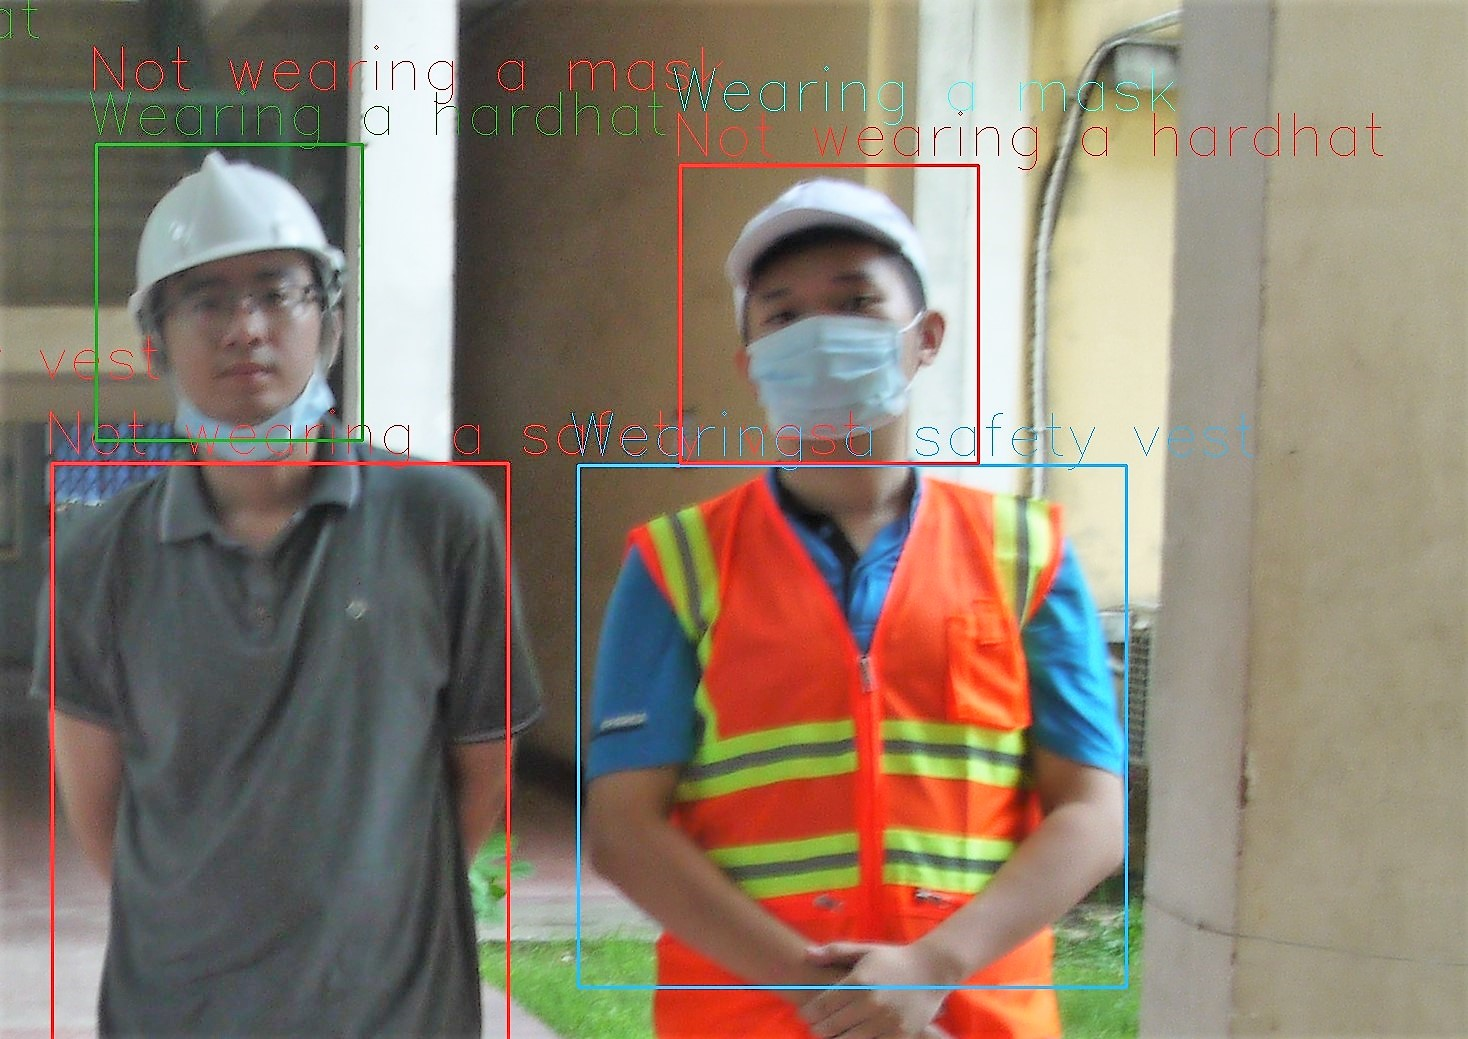
\includegraphics[scale=0.4]{images/good_hh_zoom.jpg}}
  	\caption{Mô hình có thể phân biệt tốt giữa nón vải trắng và nón bảo hiểm trắng ở khoảng cách 3m.}
  	\label{fig:good_hh_zoom}
\end{figure}
\begin{figure}[ht!]
	\centerline{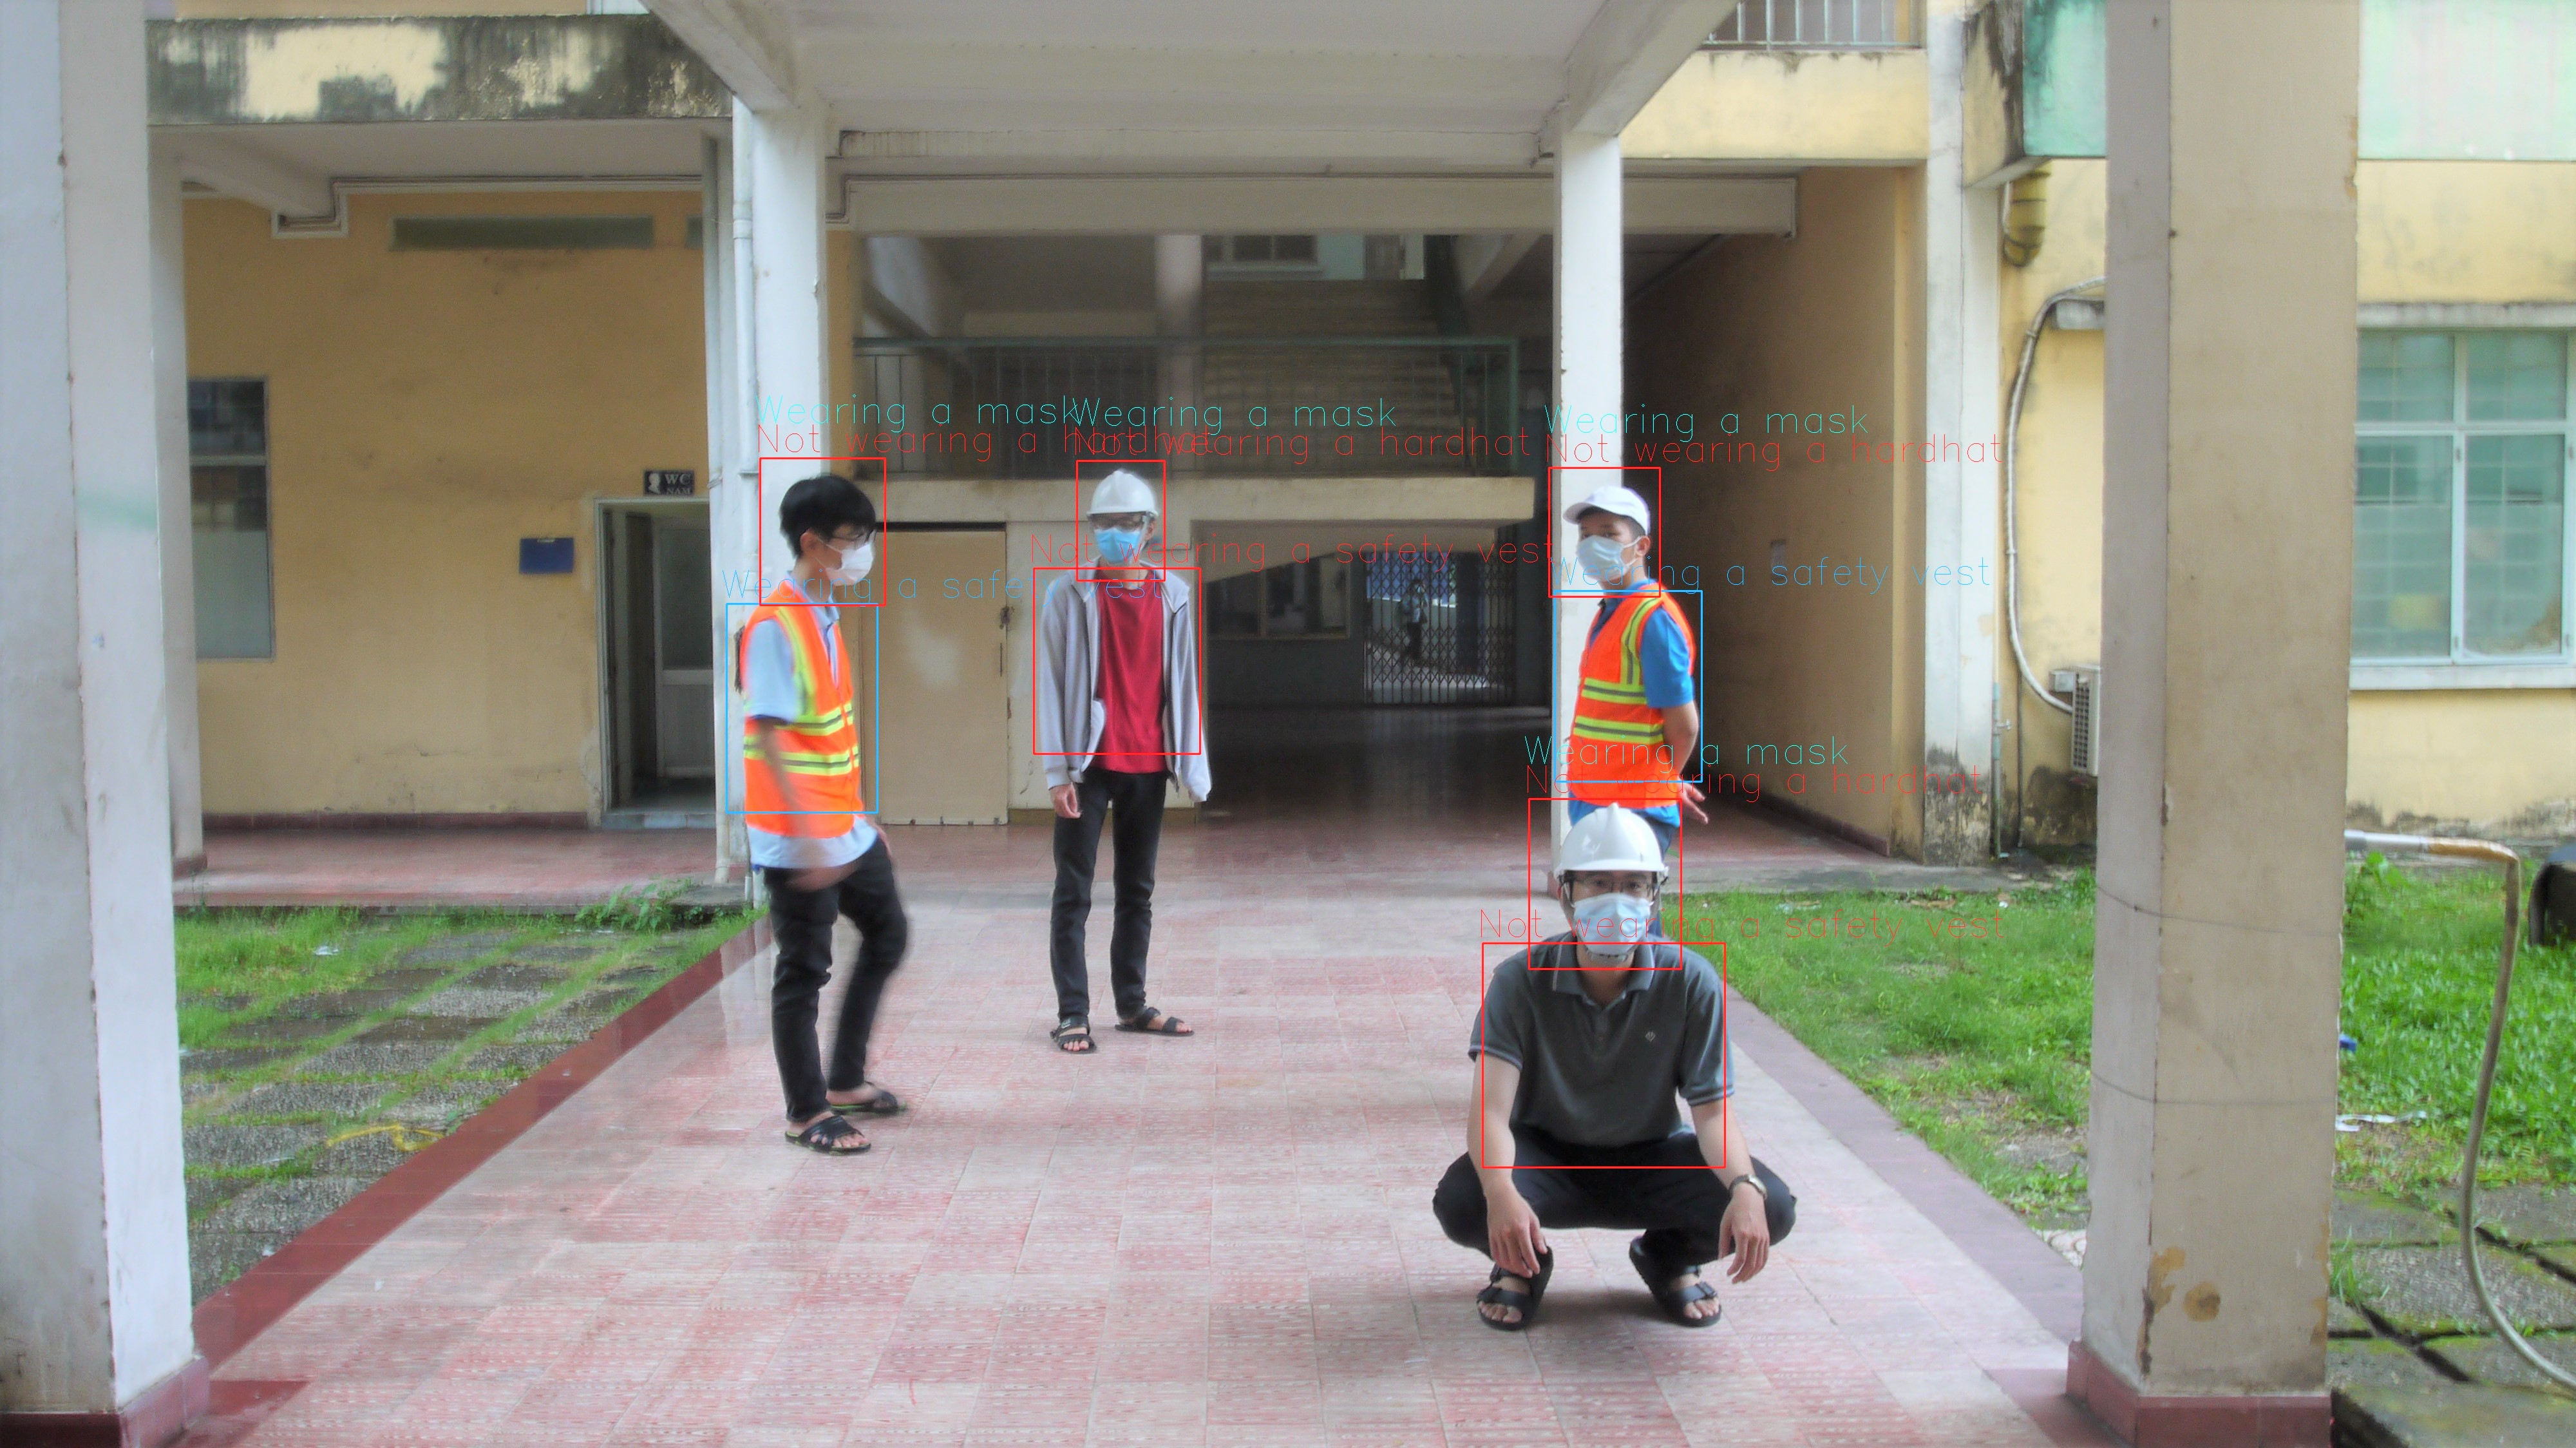
\includegraphics[scale=0.1]{images/good_hh_6m.jpg}}
  	\caption{Dự đoán của mô hình ở khoảng cách 6m.}
  	\label{fig:good_hh_6m}
\end{figure}
\begin{figure}[ht!]
	\centerline{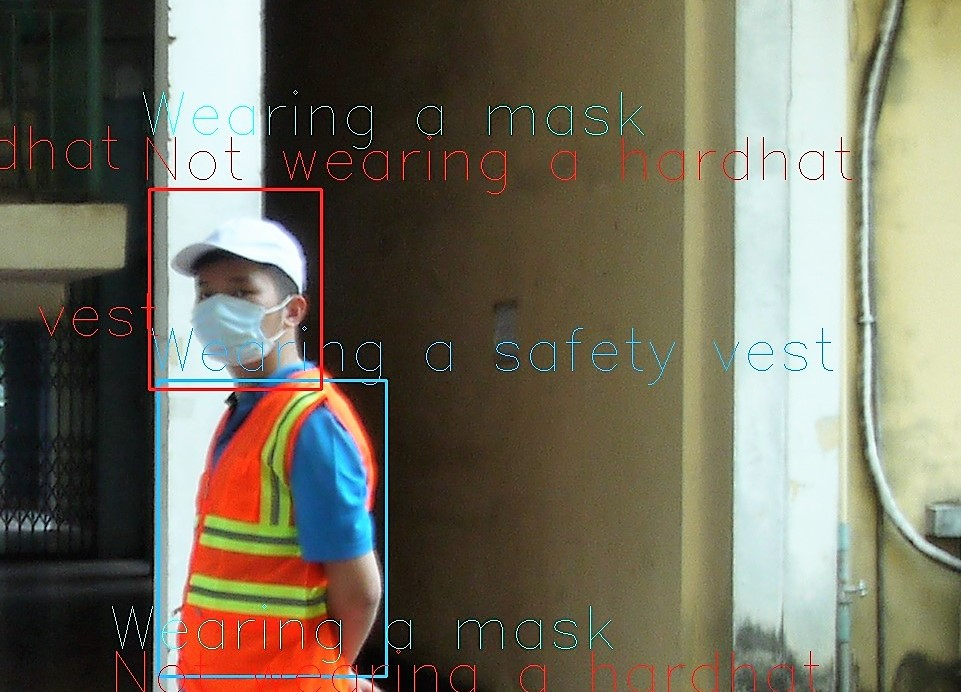
\includegraphics[scale=0.4]{images/good_hh_6m_zoom.jpg}}
  	\caption{Mô hình có thể phân biệt tốt giữa nón vải trắng và nón bảo hiểm trắng ở khoảng cách 6m.}
  	\label{fig:good_hh_6m_zoom}
\end{figure}
\begin{figure}[ht!]
	\centerline{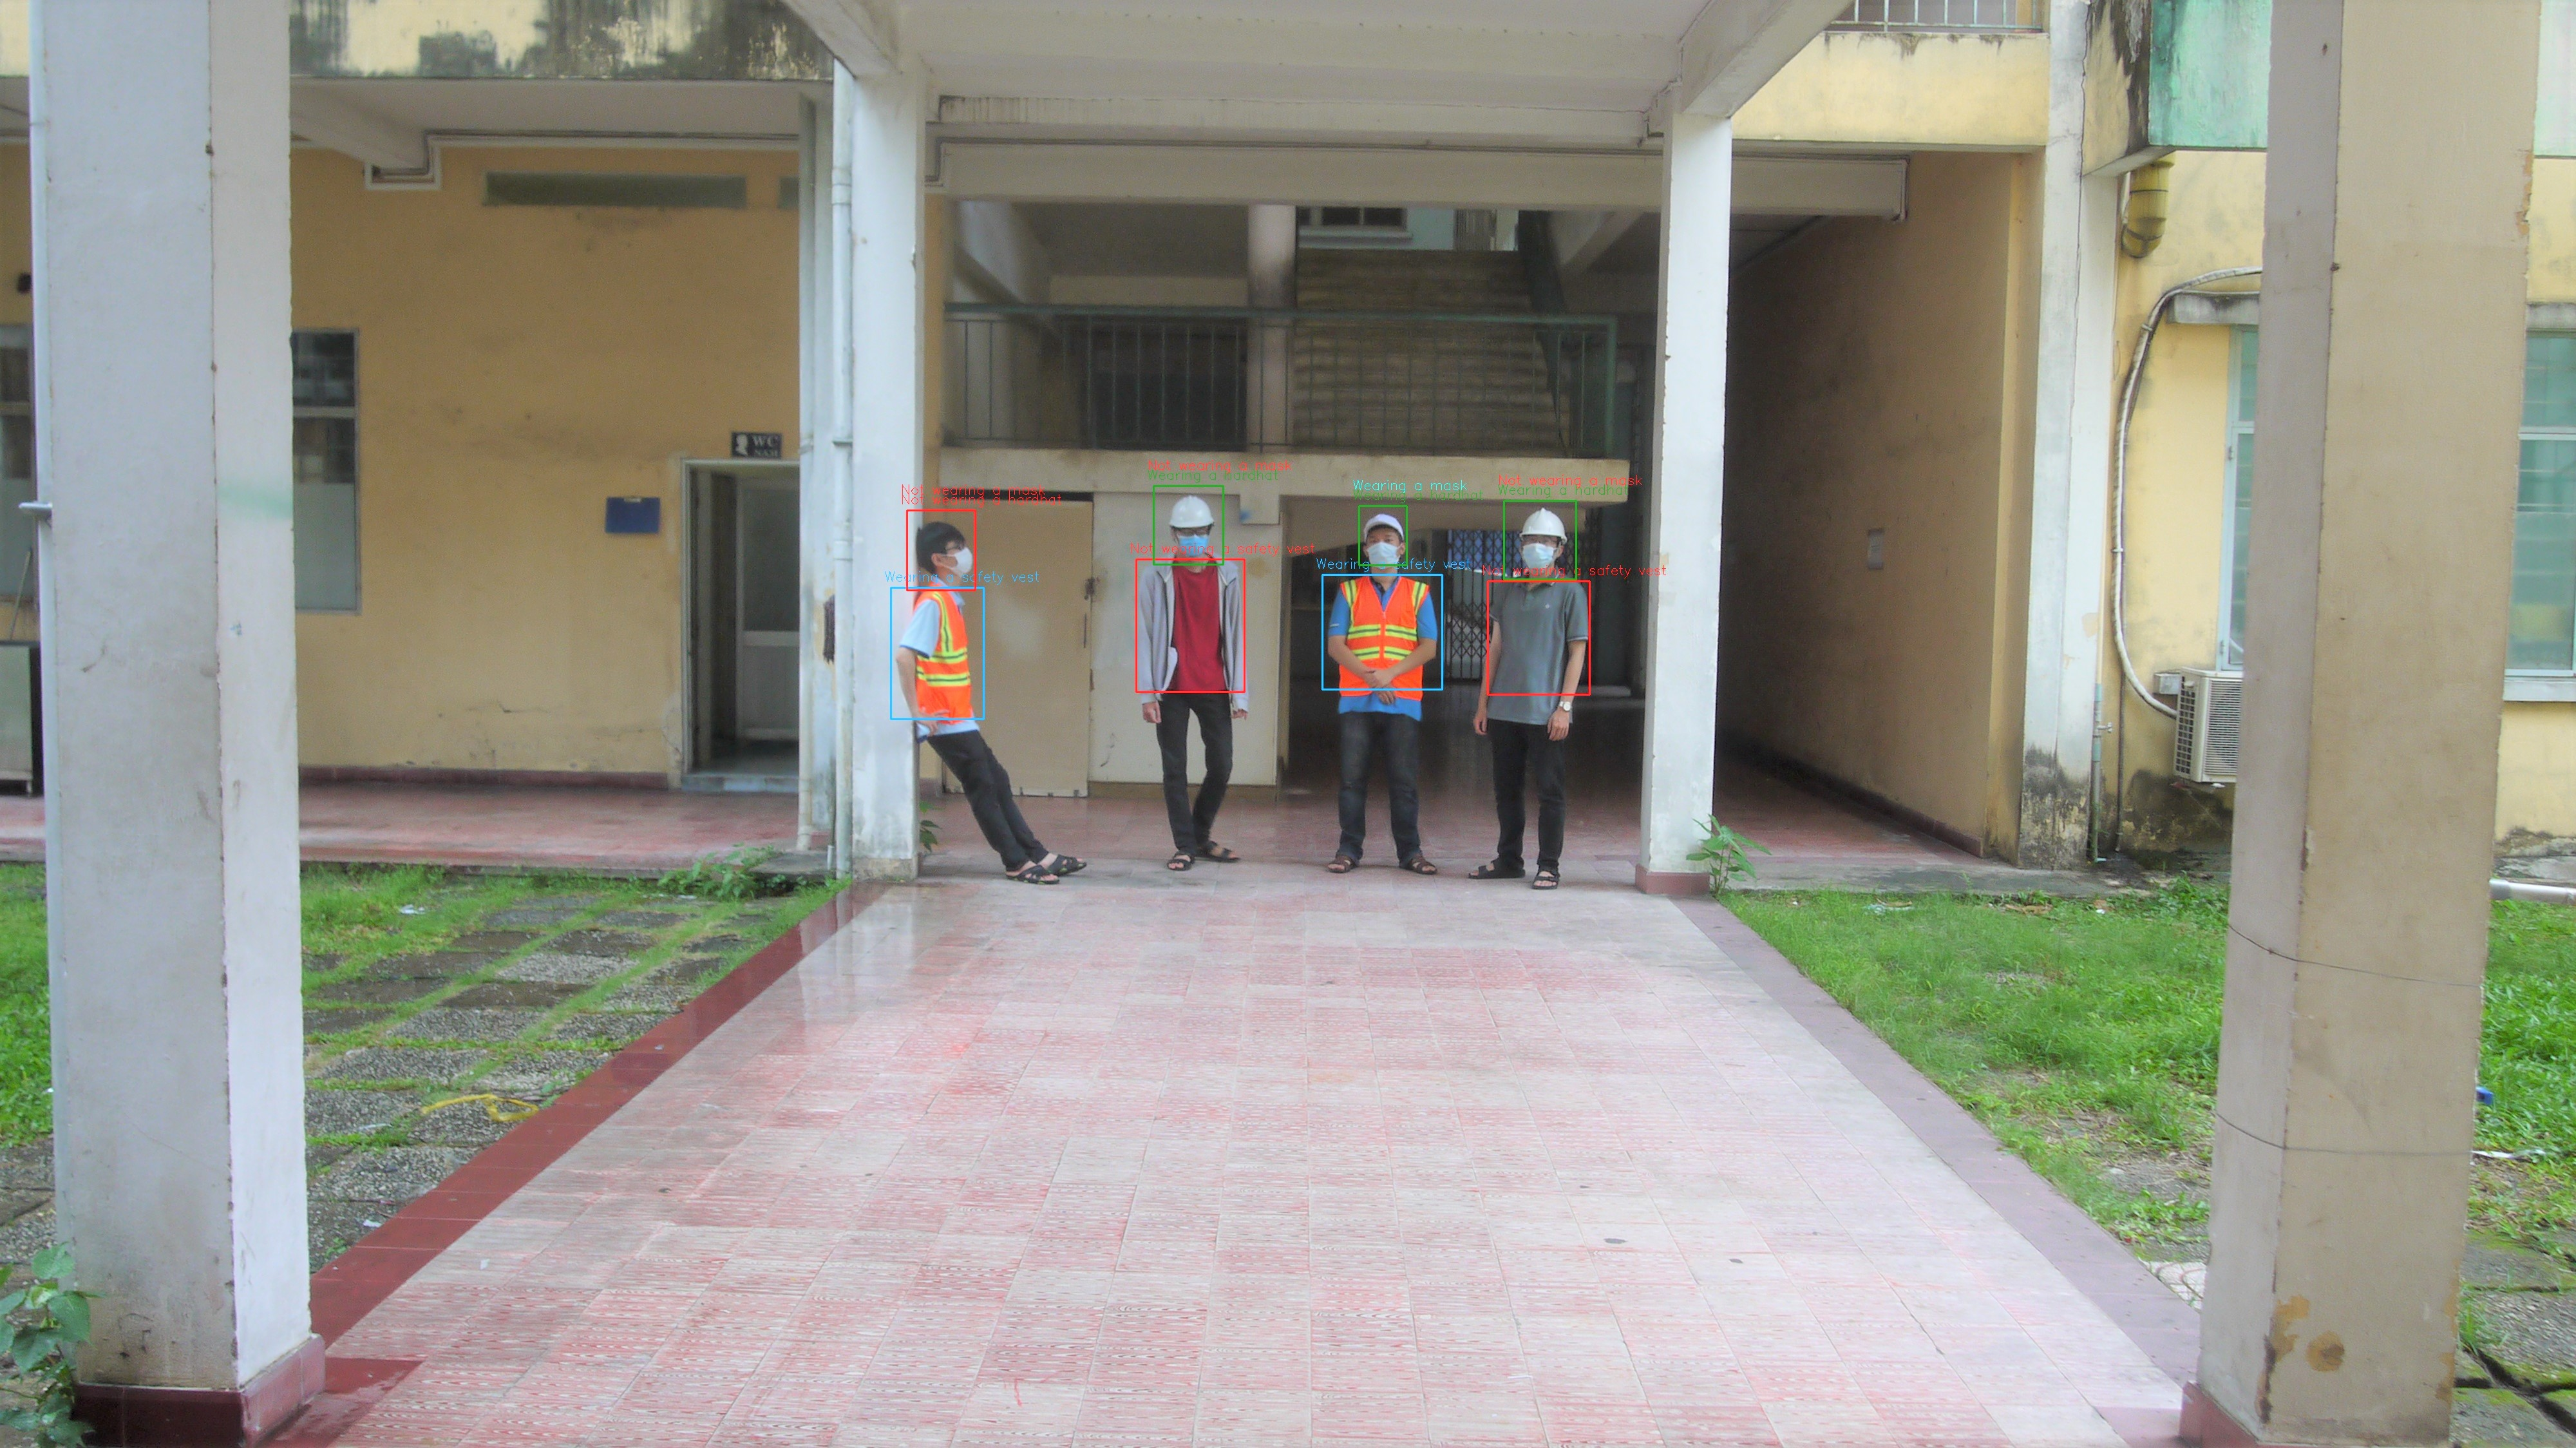
\includegraphics[scale=0.1]{images/bad_hh_9m.jpg}}
  	\caption{Dự đoán của mô hình ở khoảng cách 9m.}
  	\label{fig:good_hh_9m}
\end{figure}
\begin{figure}[ht!]
	\centerline{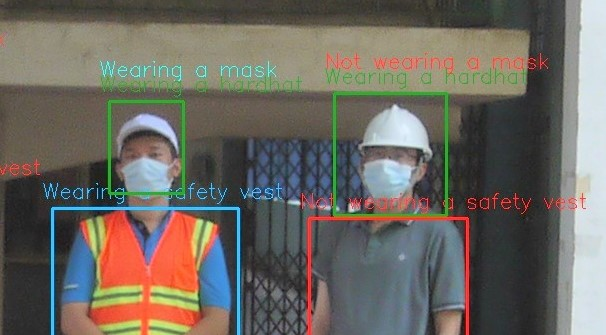
\includegraphics[scale=0.8]{images/bad_hh_9m_zoom.jpg}}
  	\caption{Mô hình không thể phân biệt tốt giữa nón vải trắng và nón bảo hiểm trắng ở khoảng cách 9m.}
  	\label{fig:good_hh_9m_zoom}
\end{figure}

\subsubsection{Thử nghiệm khả năng nhận diện của mô hình vơi các trường hợp sử dụng sai cách các thiết bị bảo hộ}
Việc sử dụng các thiết bị bảo hộ sai cách cũng nguy hiểm giống như việc không sử dụng thiết bị bảo hộ, do đó không chỉ cần phải phân biệt giữa có sử dụng hay không mà mô hình còn phải có thể phân biệt được giữa sử dụng đúng và sai trang thiết bị bảo hộ. Trong trường hợp này, chủ thể sẽ đeo khẩu trang sai cách hoặc mặc áo phản quang sai cách để kiểm tra khả năng nhận diện của mô hình.

\emph{Trường hợp 1}: Việc đeo khẩu trang sai cách sẽ được thực hiện thông qua hai trường hợp, một là đeo khẩu trang hở mũi - hình \ref{fig:bad_mask_nose}, hai là đeo khẩu trang hở miệng - hình \ref{fig:bad_mask_mouth}. Các kết quả dự đoán được thực hiện trên hình ở khoảng cách $3$m.
\begin{figure}[ht!]
	\centerline{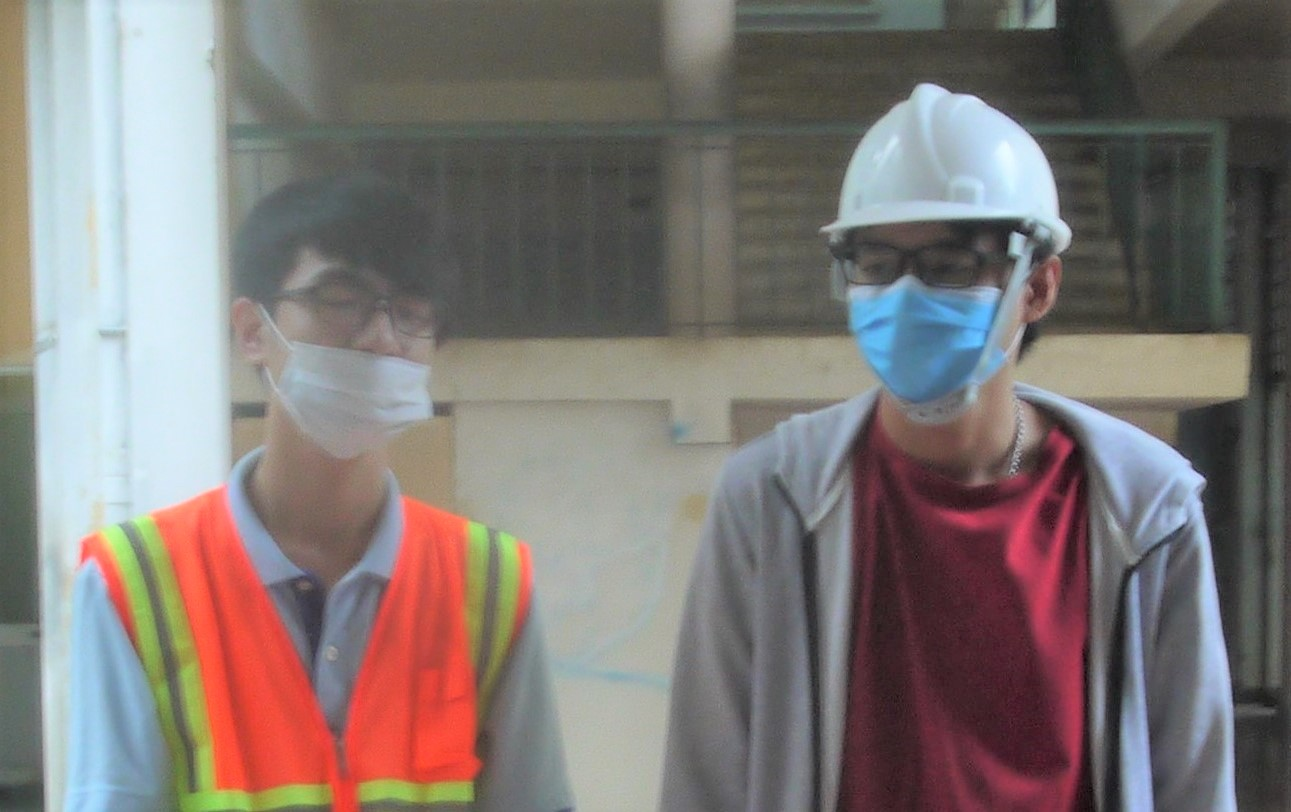
\includegraphics[scale=0.7]{images/bad_mask_nose.jpg}}
  	\caption{Chủ thể (bên trái) đeo khẩu trang không che kín mũi ở khoảng cách 3m.}
  	\label{fig:bad_mask_nose}
\end{figure}
\begin{figure}[ht!]
	\centerline{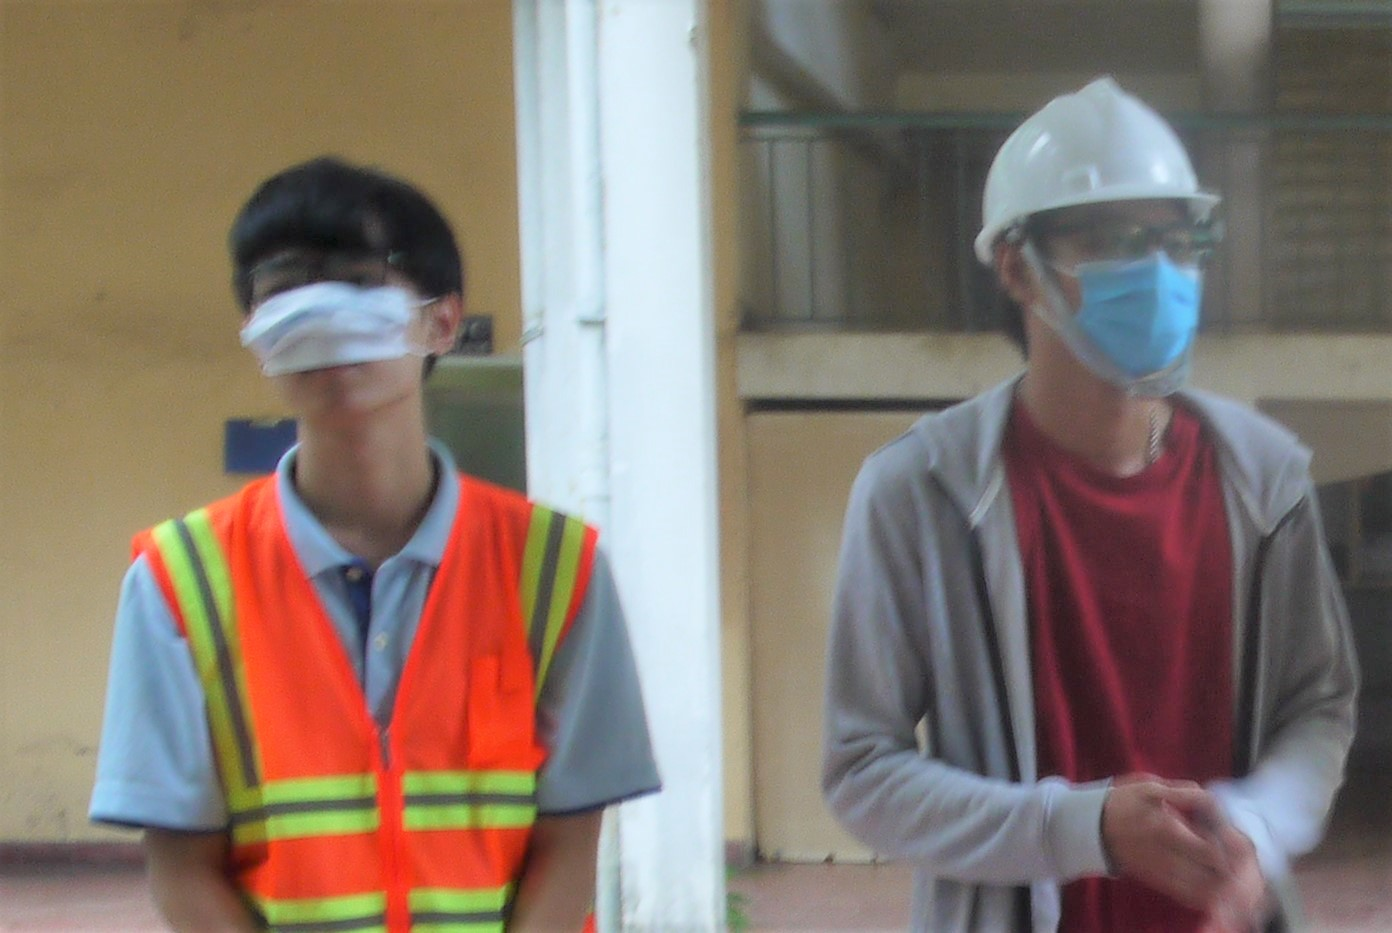
\includegraphics[scale=0.65]{images/bad_mask_mouth.jpg}}
  	\caption{Chủ thể (bên trái) đeo khẩu trang không che kín miệng ở khoảng cách 3m.}
  	\label{fig:bad_mask_mouth}
\end{figure}
\emph{Kết quả}: Mô hình không thể phân biệt được trường hợp đeo khẩu trang sai khi chủ thể đeo khẩu trang để hở mũi - hình \ref{fig:bad_mask_nose_pred}. Mô hình có thể phân biệt tốt trong trương hợp đeo khẩu trang sai khi chủ thể đeo khẩu trang hở miệng - hình \ref{fig:bad_mask_mouth_pred}.
\begin{figure}[ht!]
	\centerline{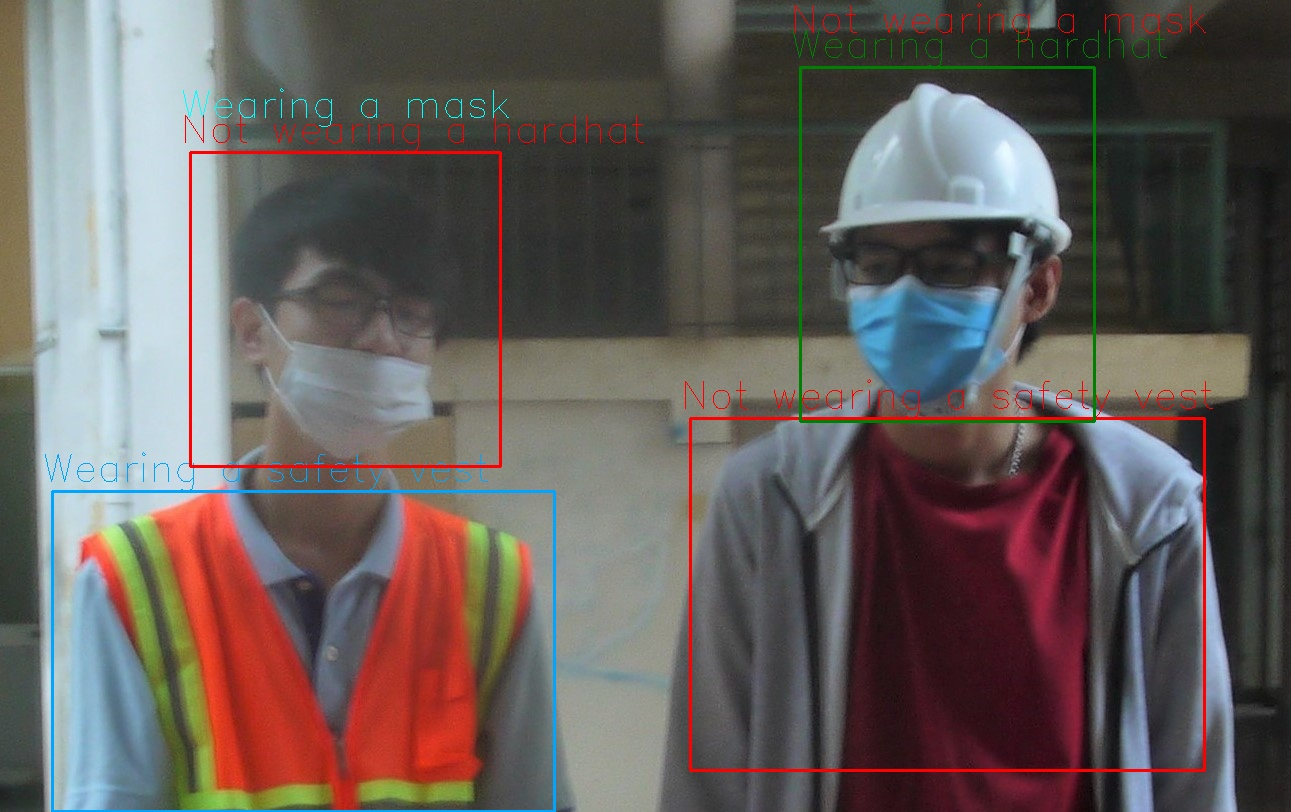
\includegraphics[scale=0.3]{images/bad_mask_nose_pred.jpg}}
  	\caption{Kết quả dự đoán không tốt với chủ thể (bên trái) đeo khẩu trang không che kín mũi ở khoảng cách 3m.}
  	\label{fig:bad_mask_nose_pred}
\end{figure}
\begin{figure}[ht!]
	\centerline{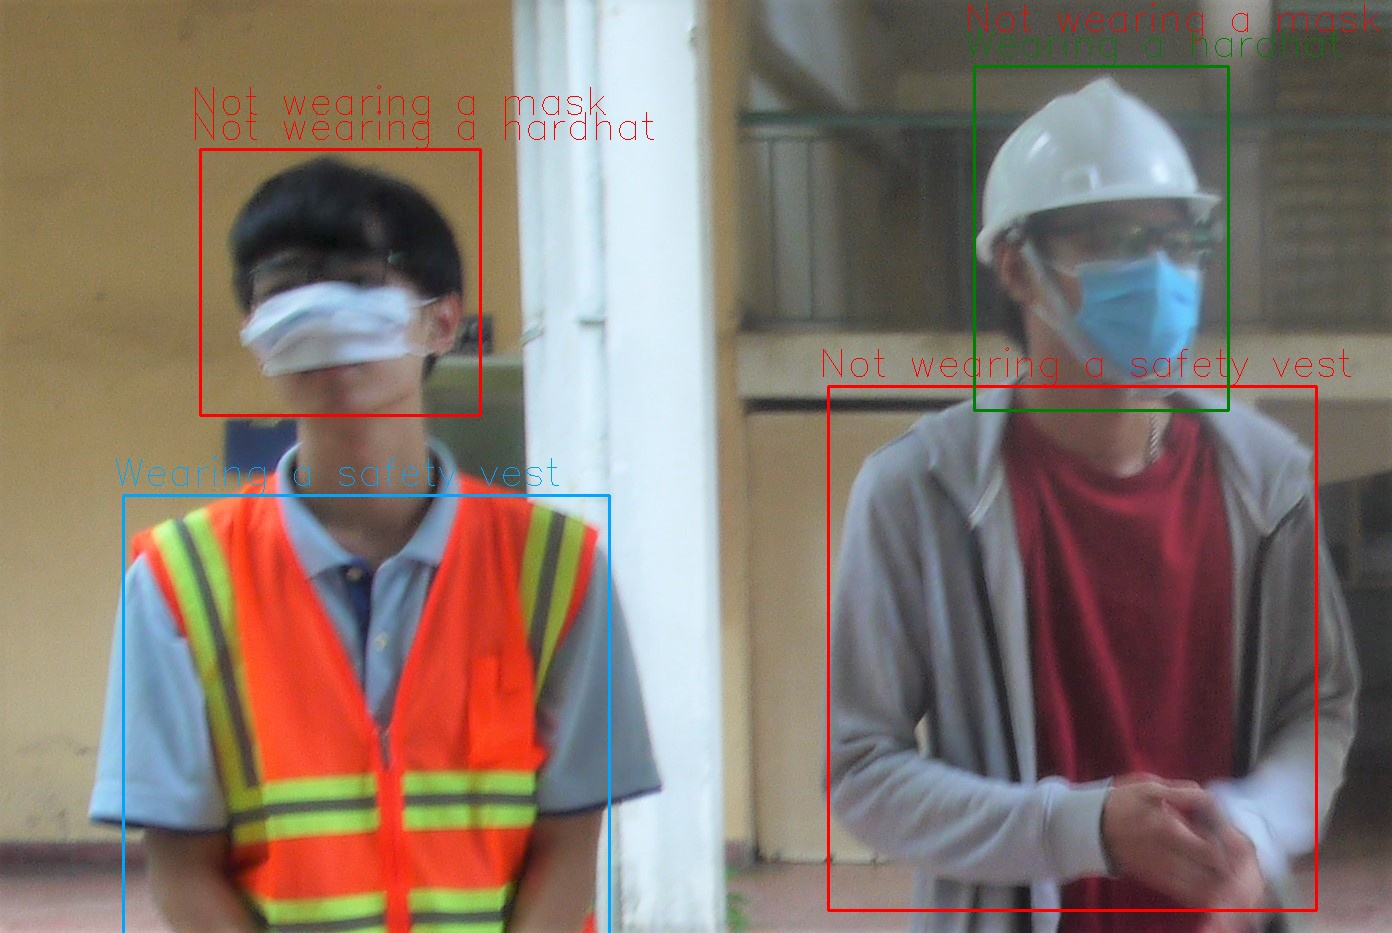
\includegraphics[scale=0.3]{images/bad_mask_mouth_pred.jpg}}
  	\caption{Kết quả dự đoán tốt với chủ thể (bên trái) đeo khẩu trang không che kín miệng ở khoảng cách 3m.}
  	\label{fig:bad_mask_mouth_pred}
\end{figure}

\emph{Trường hợp 2}: Việc mặc áo bảo hộ sai cách sẽ được thực hiện bằng cách chỉ đặt áo lên người mà không thật sự mặc hoặc mặc nhưng không cài vào đúng cách như trong hình \ref{fig:bad_sv}, việc này có thể khiến áo dễ mắc vào các thiết bị phương tiện đang hoạt động và gây ra các tai nạn đáng tiếc. Các kết quả dự đoán được thực hiện trên hình ở khoảng cách $3$m.
\begin{figure}[ht!]
	\centerline{\includegraphics[scale=0.25]{images/bad_sv.jpg}}
  	\caption{Hai chủ thể (bên trái ngoài cùng) mặc áo bảo hộ sai cách ở khoảng cách 3m.}
  	\label{fig:bad_sv}
\end{figure}
\emph{Kết quả}: Mô hình có thể phân biệt được các trường hợp mặc sai áo bảo hộ ở phần lớn các trường hợp như trên hình \ref{fig:bad_sv_pred_1} và \ref{fig:bad_sv_pred_2}. Tuy nhiên ở một vài góc chụp như trên hình \ref{fig:bad_sv_pred_3} thì mô hình không thể nhận diện được chính xác. Điều này có thể không phải là nhược điểm lớn vì khi nhận diện trong thực tế thì mô hình sẽ nhận diện liên tục qua nhiều khung hình do đó những trường hợp mặc sai khi bị bỏ qua ở khung hình này thì sẽ được phát hiện trong khung hình khác.
\begin{figure}[ht!]
	\centerline{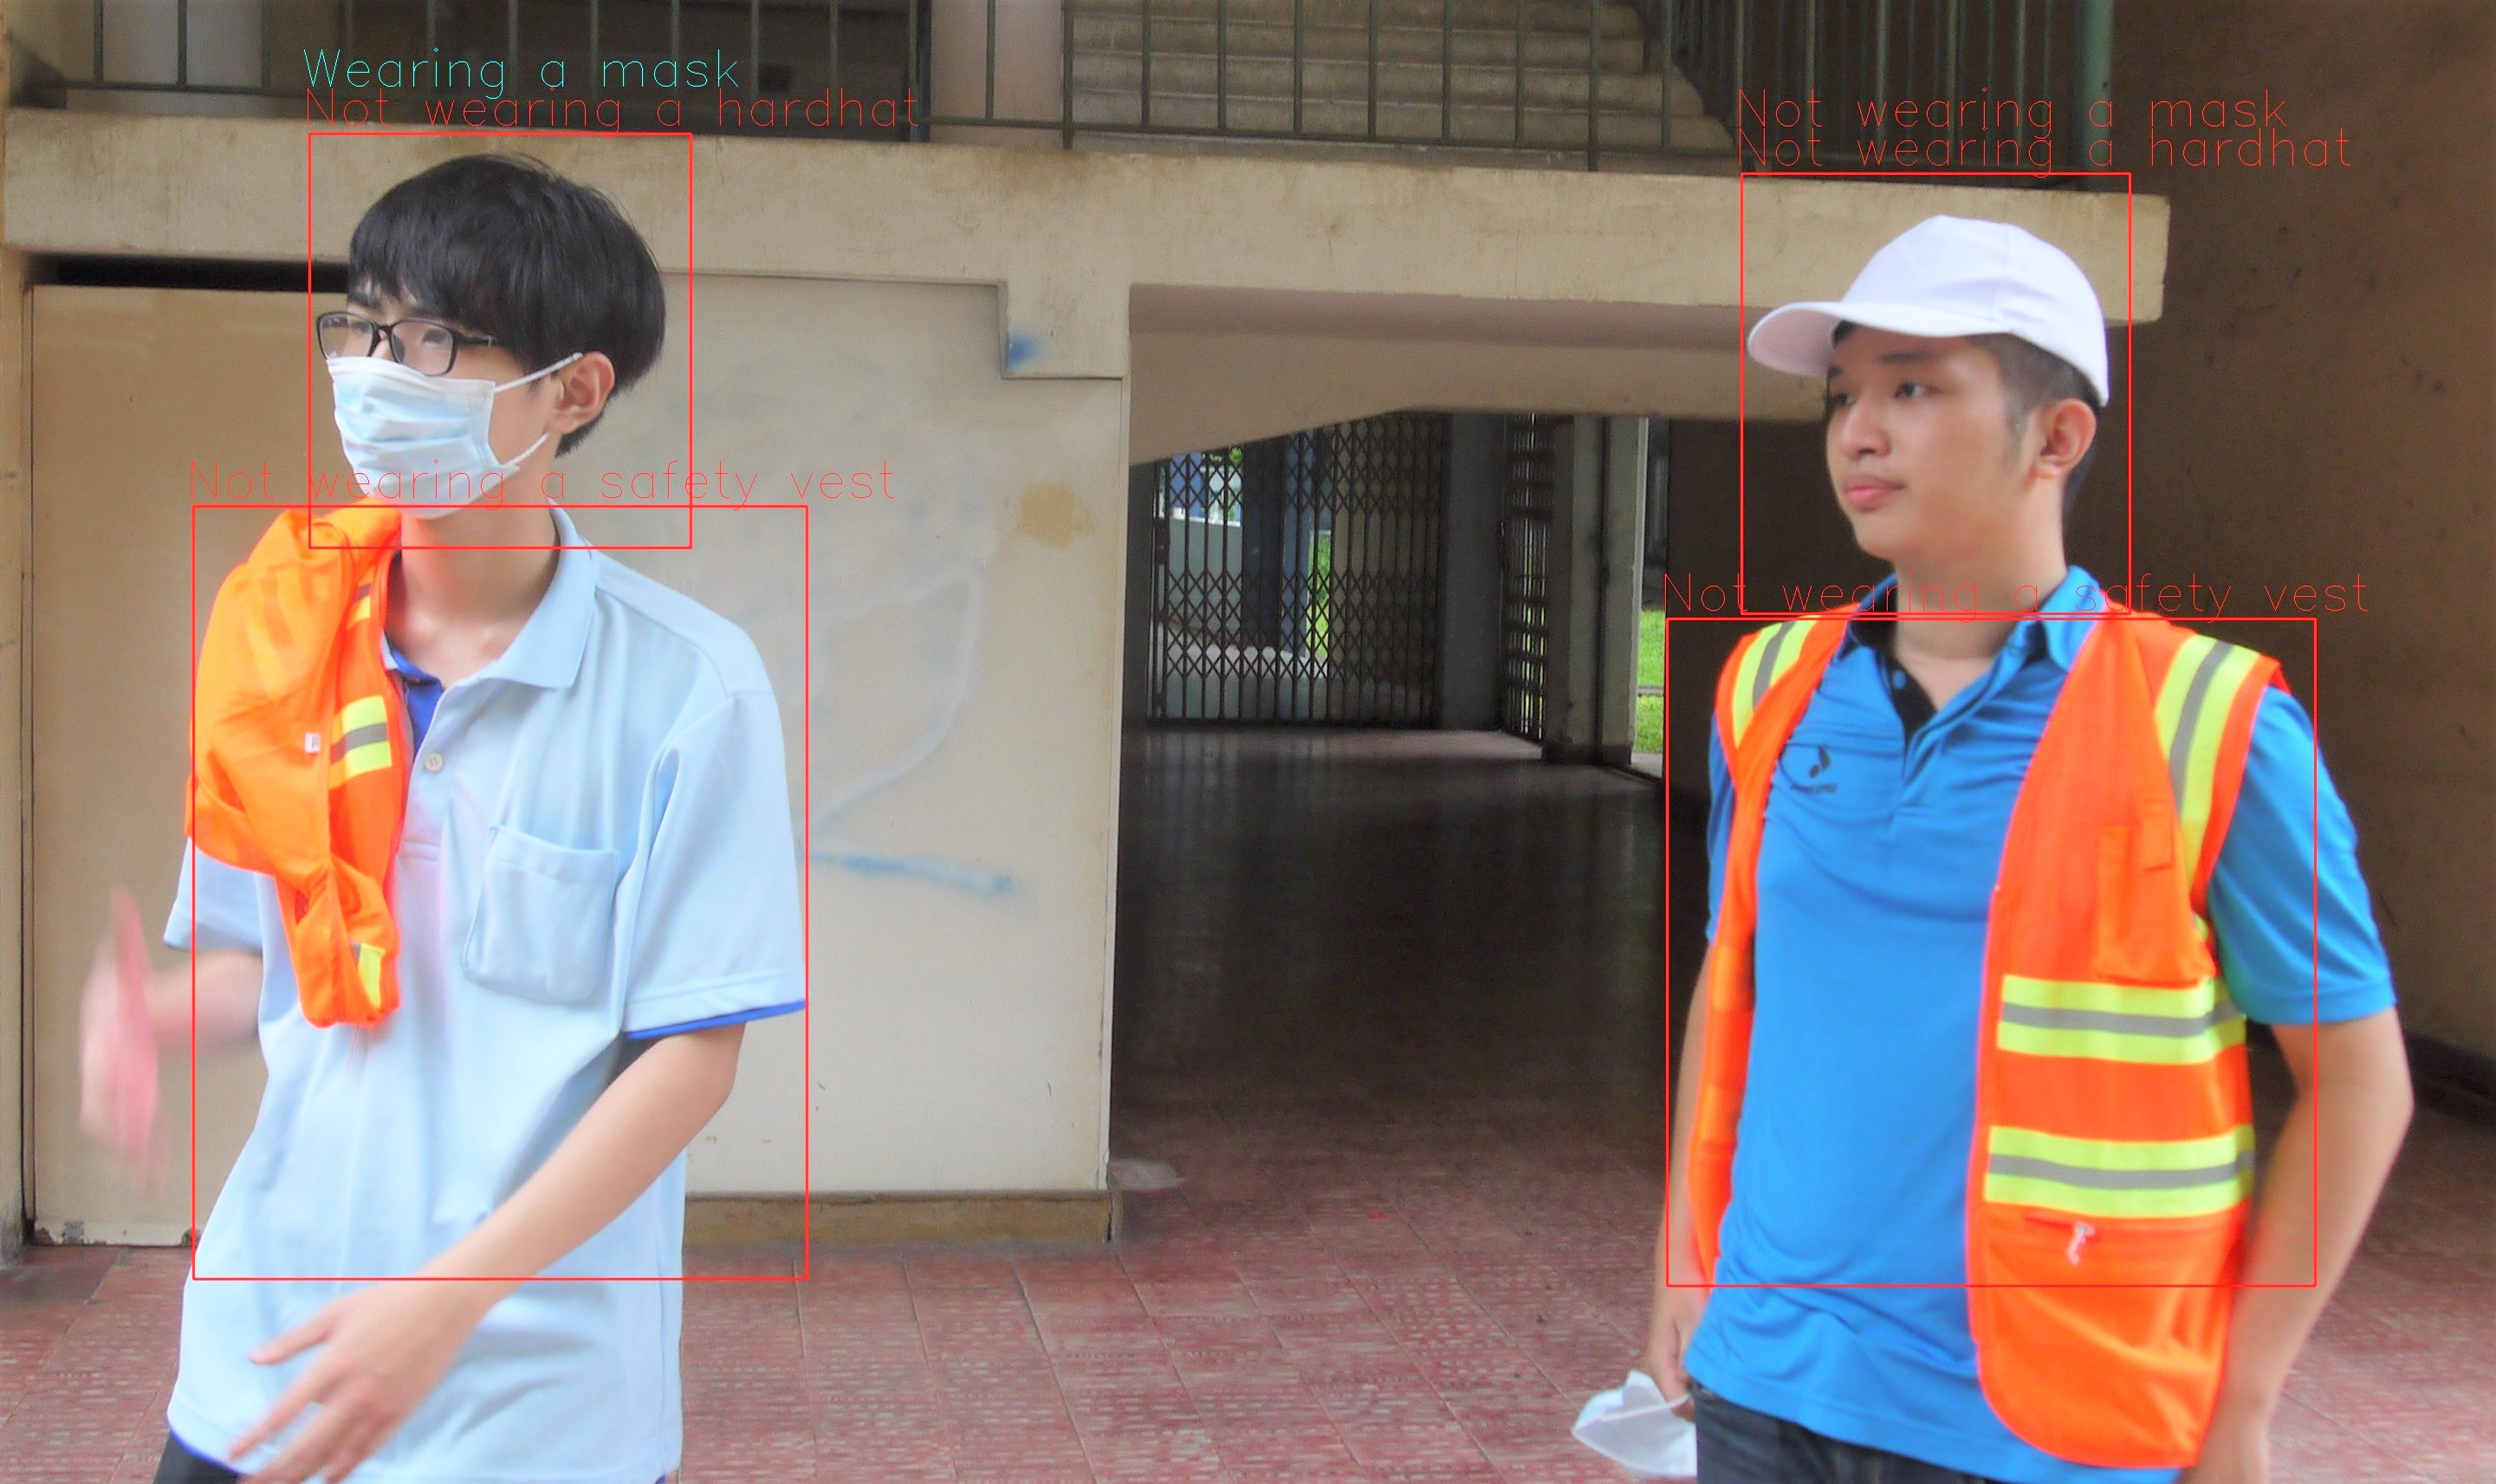
\includegraphics[scale=0.18]{images/bad_sv_predict_2.jpg}}
  	\caption{Kết quả dự đoán tốt với hai chủ thể mặc áo bảo hộ sai cách ở khoảng cách 3m.}
  	\label{fig:bad_sv_pred_1}
\end{figure}
\begin{figure}[ht!]
	\centerline{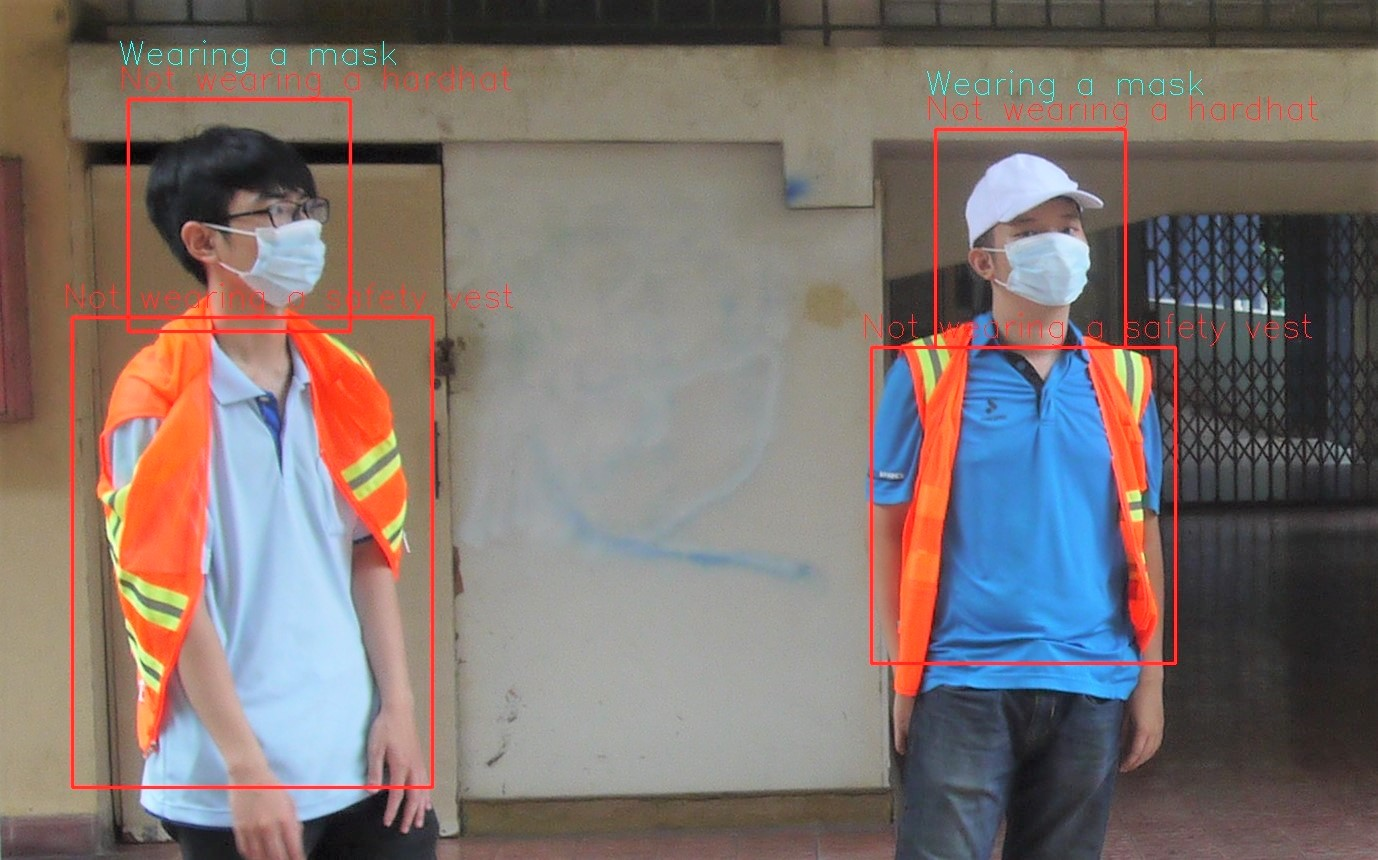
\includegraphics[scale=0.35]{images/bad_sv_predict_3.jpg}}
  	\caption{Kết quả dự đoán tốt với hai chủ thể mặc áo bảo hộ sai cách (góc máy khác) ở khoảng cách 3m.}
  	\label{fig:bad_sv_pred_2}
\end{figure}
\begin{figure}[ht!]
	\centerline{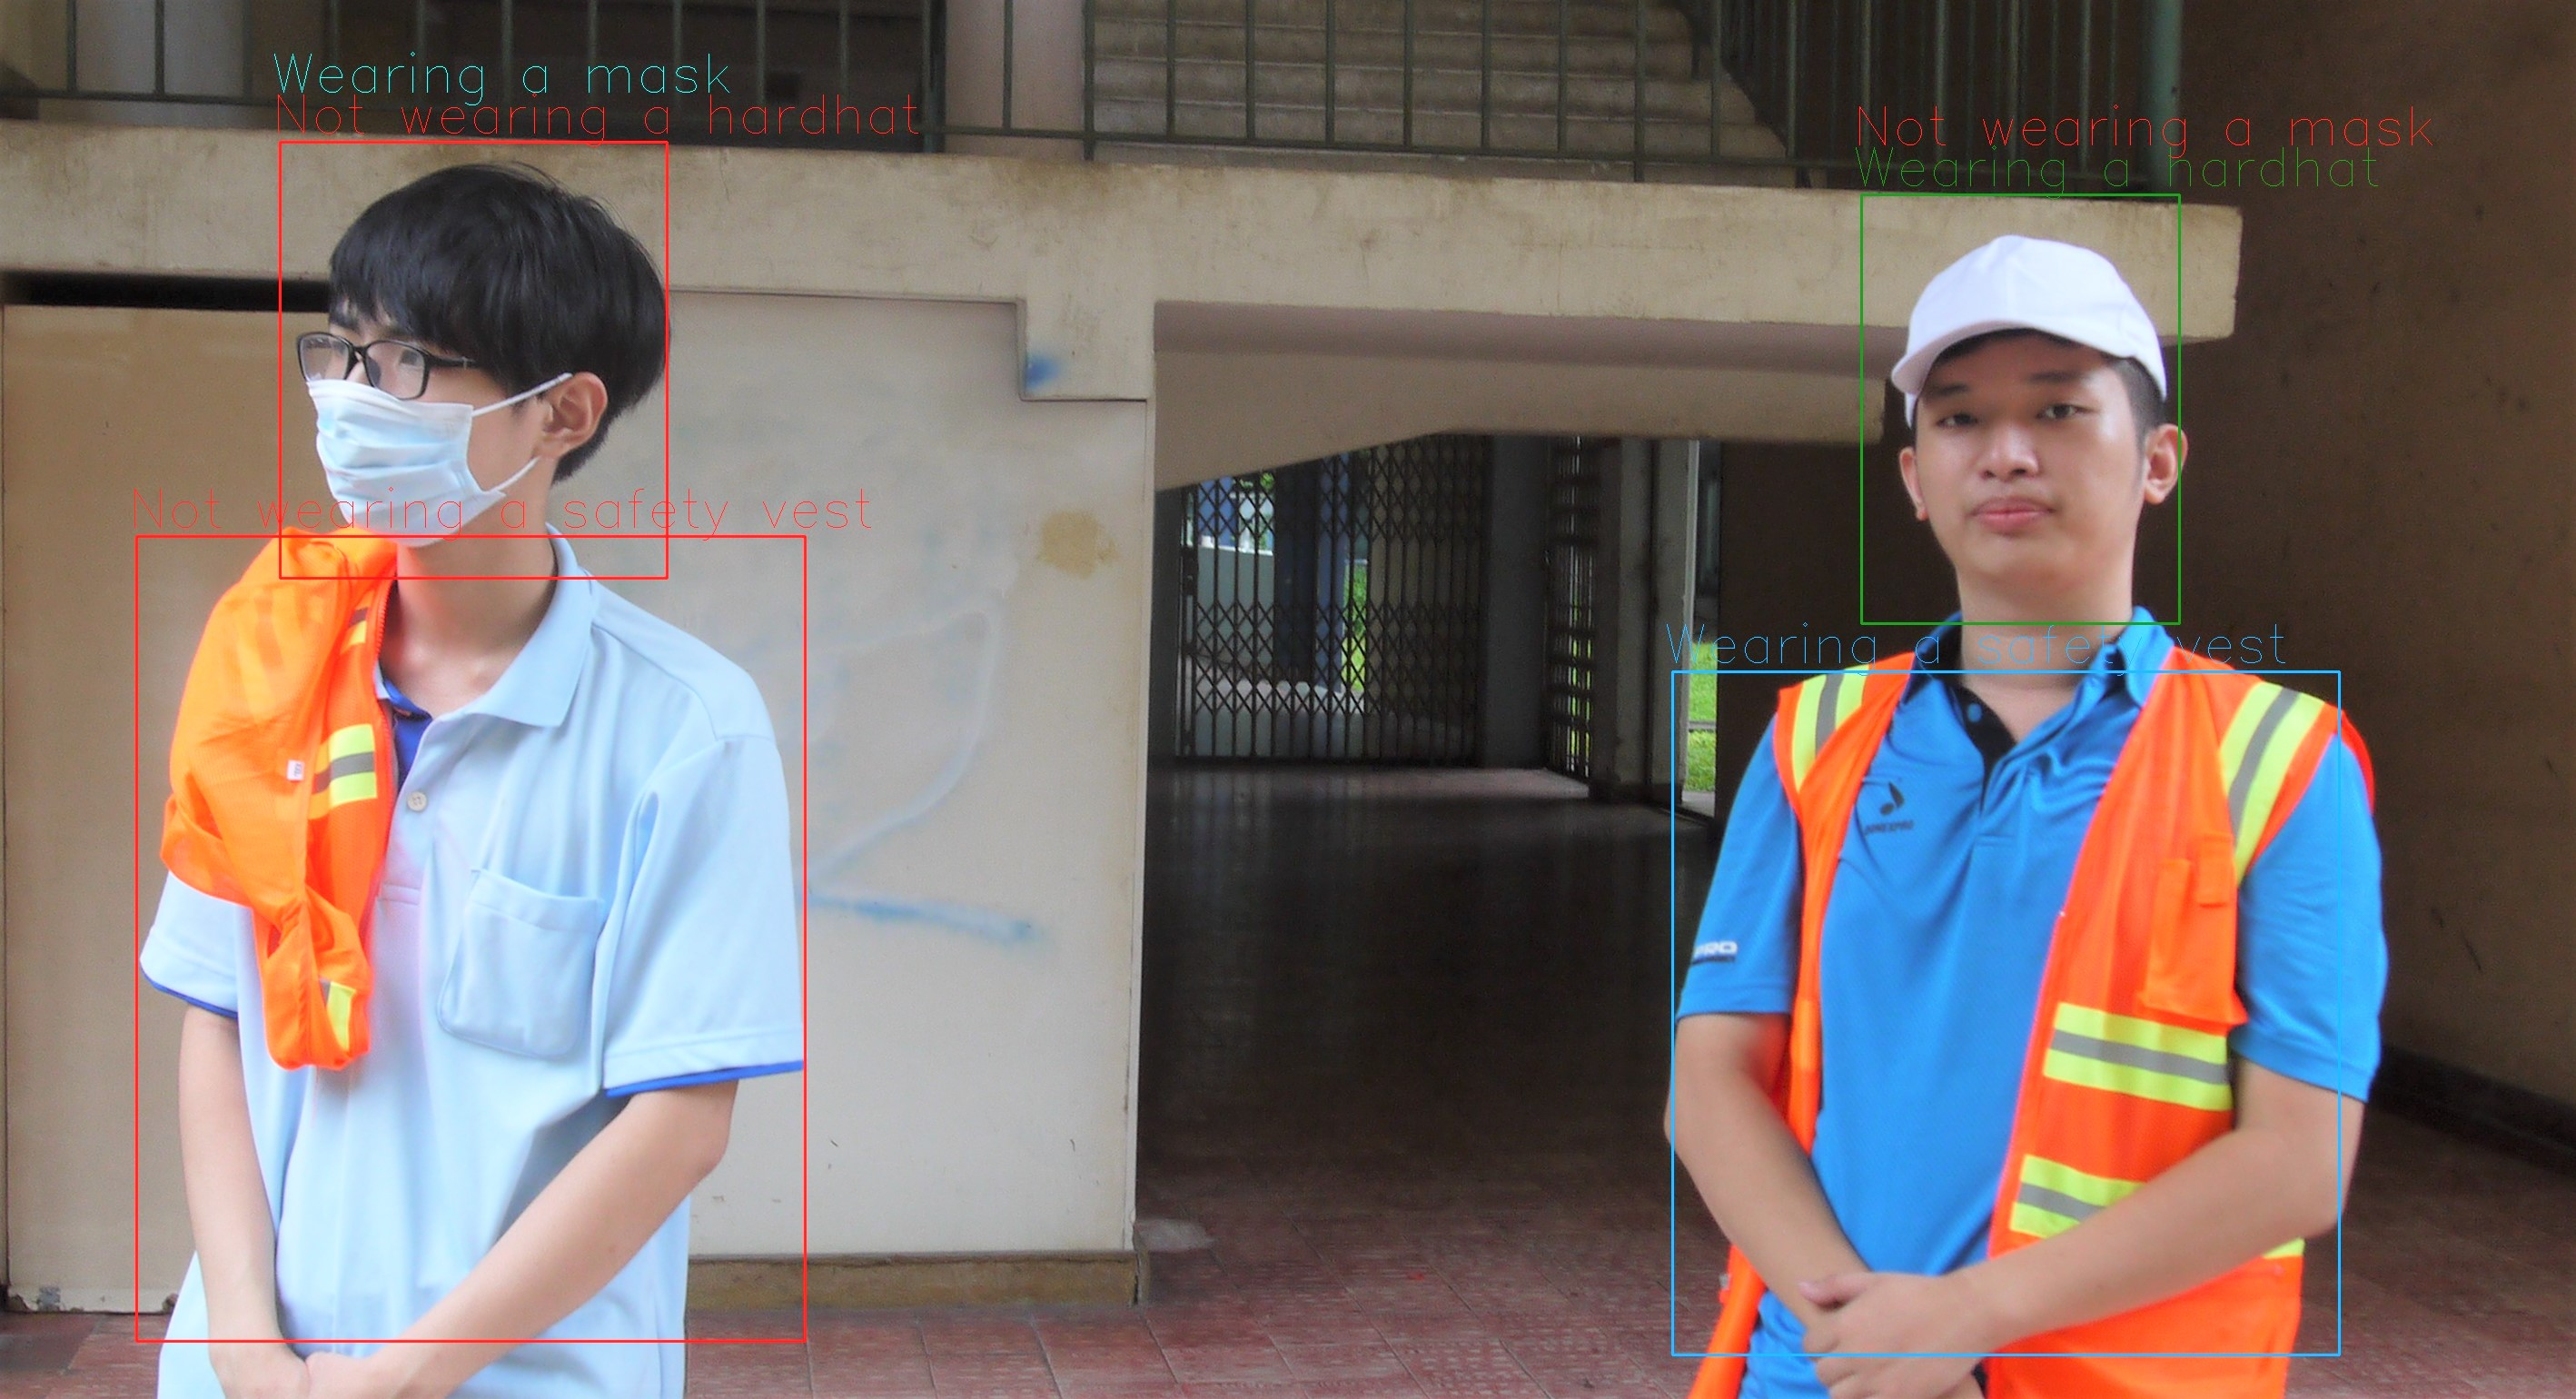
\includegraphics[scale=0.18]{images/bad_sv_predict_4.jpg}}
  	\caption{Kết quả dự đoán không tốt với hai chủ thể mặc áo bảo hộ sai cách ở khoảng cách 3m.}
  	\label{fig:bad_sv_pred_3}
\end{figure}